\documentclass{config/apuntes}

\title{Filogenia molecular}
\author{Sandra Mingo Ramírez}
\date{2024/25}
\acronym{PHYLO}

\usepackage[all]{nowidow}
\usepackage{listing}
\usepackage{color}
\usepackage{tabularx}
\usepackage{multirow}
\usepackage{makecell}
\usepackage{amsmath}
\usepackage{array}

\begin{document}

\begin{abstract}
La filogenia molecular es la rama de la filogenia que analiza las diferencias moleculares hereditarias en las secuencias de ADN, ARN y proteínas para obtener información sobre las relaciones evolutivas de un organismo. El resultado de un análisis filogenético molecular se expresa en un árbol filogenético.
\end{abstract}

\pagestyle{plain}

\maketitle

\tableofcontents

%Examen de teoría 33% (algunas tipo test y otras de respuesta corta de conceptos), trabajo final 66%
%Para aprobar la asignatura es obligatorio obtener una nota mayor o igual a 5 puntos tanto en la parte de teoría como en el trabajo final.
%no va a haber fórmulas ni siglas, pero sí que en función de unos datos se hagan unas metodologías u otras. Un árbol cae fijo, y la relación entre los taxones también. Va a tirar más hacia la interpretación; calcular el árbol más parsimonioso y por qué, el árbol que se genera con los métodos no es el más probable, es el que mejor describe los datos.

%09/09 - Patricia Álvarez
\chapter{Introducción a la filogenia: principios y conceptos}
La filogenia es la determinación de la historia evolutiva de los organismos. Así, la filogenética es el estudio de: (i) la filogenia mediante el uso de árboles filogenéticos de los distintos organismos y (ii) las relaciones entre ellos. Ha habido varias iniciativas a lo largo de la historia (como \href{http://tolweb.org}{ToL Web}) que han intentado lograr crear árboles de todas las especies, cuyo número se estima por lo bajo que ronda los 3-5 millones. Estas estimaciones sobre la biodiversidad se realizan a partir de el número de grupos clave como los escarabajos, que son el grupo con mayor número de spp., en un lugar.

La filogenia es una disciplina muy consolidada; desde sus inicios, hace aproximadamente 200 años, sus representaciones no han cambiado mucho. La filogenia trabaja con árboles evolutivos, que son las \textbf{representaciones gráficas (patrones) de las relaciones ancestro-descendientes (relaciones históricas de parentescos) entre elementos}, que pueden ser especies, secuencias de genes, etc. Entender este patrón es esencial para realizar estudios comparativos de cualquier tipo, porque existen\textbf{ dependencias estadísticas entre los elementos que comparten ancestros comunes}. Conforme pasa el tiempo, se van aplicando diferentes y nuevos modelos evolutivos y se van depurando. En ultima instancia, se obtiene una mejor aproximación cuantos más datos se añadan (tanto más especies como más secuencias) a los modelos.

La filogenia sirve, entre otros, para: 
\begin{itemize}
\item Evolución de los seres vivos
\item Genómica: se puede observar mucho más allá y establecer límites entre especies. (Ej.: la evaluación es críptica. Si nos imaginamos a unos extraterrestres, no sabrán si clasificarnos a todos los humanos como una misma especie o distintas.)
\item Ingeniería genética
\item Farmacia
\item Epidemiología: ébola, VIH-1, etc. (Ver siguiente párrafo)
\item Biología de la conservación: discernir entre poblaciones y especies importa en relación con la clasificación de los espacios protegidos.
\item Control de plagas
\item Lingüística
\end{itemize}

La filogenética puede ser estudiada de diversas maneras. A menudo ha sido estudiada utilizando \textbf{registros fósiles}, que contienen información sobre la morfología de los antepasados de las especies actuales y la cronología de sus divergencias. Esto permite datar las filogenias. Sin embargo, el uso de registros fósiles presenta muchas limitaciones: pueden estar disponibles sólo para determinadas especies, los datos existentes de fósiles pueden estar fragmentados, la recolección de datos está limitada por la abundancia, hábitat, rango geográfico y otros factores; y las descripciones de los rasgos morfológicos son a menudo ambiguas (múltiples factores genéticos). Por todo esto, utilizar registros fósiles para determinar relaciones filogenéticas puede producir \textbf{sesgos}. Además, los fósiles de microorganismos son prácticamente inexistentes imposibilitando el uso de este enfoque. Afortunadamente, los \textbf{datos moleculares} que están en la forma de secuencias de ADN o de proteínas pueden ser también muy útiles para proporcionar una perspectiva de la evolución de los organismos, como el ARN 16S. Debido a que los genes son el medio para registrar las mutaciones acumuladas, éstos pueden servir como "fósiles moleculares". A través del análisis comparativo de secuencias de ADN de una serie de organismos relacionados, la historia evolutiva de los genes e incluso de los organismos puede ser revelada. La ventaja de utilización de datos moleculares es que son más numerosos que los registros fósiles y más fáciles de obtener. Además, no hay ningún sesgo de muestreo, como el que hay en los registros fósiles reales. Por tanto, es posible construir árboles filogenéticos más precisos y robustos utilizando datos moleculares. Como ejemplos, la filogenética se ha usado para datar y ubicar el origen del ébola en el brote de 2014 o el paciente 0 del VIH-1 en 1970.

Las filogenias, al ser una reconstrucción de la evolución de los caracteres, se construyen a partir de un registro/evidencias indirecto/as del proceso evolutivo. Por tanto, se deben realizar test de homología comprobar que los caracteres son comparables entre sí al compartir un origen común (homologías) y discernirlas de las homoplasias. De esa forma se obtiene información para construir clasificaciones y hacer predicciones dentro de un marco temporal cuando es posible obtenerlo.

\section{Conceptos básicos}
Los árboles filogenéticos suelen ser binarios, estando compuestos por \textbf{nodos externos o terminales} y \textbf{nodos internos} unidos por \textbf{ramas} que parten de una \textbf{raíz}. A través de las diferentes ramas se van reconstruyendo las relaciones entre las especies. Los \textbf{nodos internos son hipótesis evolutivas de posibles ancestros comunes} de los cuales normalemente faltan datos para confirmar o descartar la teoría. En las distintas ramas se pueden representar la transformación de caracteres que aparecen a nivel genético y que se transmiten por herencia.  

\begin{figure}[htbp]
\centering
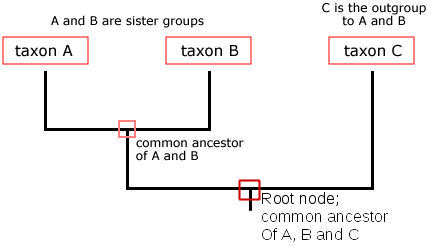
\includegraphics[width=0.5\linewidth]{figs/taxon-tree.png}
\caption{Partes de un árbol filogenético.}
\end{figure}

Se denominan \textbf{grupos hermanos} a los nodos terminales que parten de un mismo nodo interno, es decir, dos taxones que compartan un ancestro común no compartido por ningún otro taxón. El \textbf{grupo externo (outgroup)} es aquel que se encuentra más alejado y parte de una rama distinta desde la raíz. Normalmente, este outgroup se elige arbitrariamente para poder colocar la raíz donde se estima correcto. Todas las especies que se desarrollan desde una rama de la raíz se denomina \textbf{grupo interno o ingroup}. 

Los árboles filogenéticos se pueden representar sin enraizar o enraizado. Un árbol filogenético sin raíz no asume conocimiento de un ancestro común, solo posiciones de los taxones para mostrar sus relaciones relativas (no hay dirección de un camino evolutivo). Para describir la dirección de la evolución se necesita un árbol filogenético con raíz donde todas las secuencias bajo estudio tienen un ancestro o nodo raíz común (más informativo). Mientras que los árboles filogenéticos se centran en las relaciones evolutivas entre diferentes especies, las redes haplotípicas son representaciones gráficas sobre las relaciones evolutivas entre las diferentes poblaciones.

A la hora de visualización, hay varias formas de representar los árboles filogenéticos. Los distintos elementos no tienen un orden concreto; da igual si en un árbol los nodos terminales están en distinto orden mientras que las ramas sigan el mismo camino. En general, se suelen poner los nodos terminales de manera que sea más fácil de leer a simple vista.

\begin{figure}[htbp]
\centering
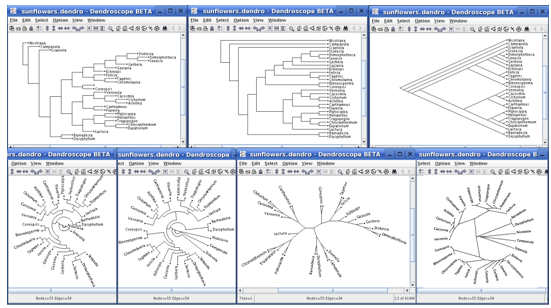
\includegraphics[width=0.5\linewidth]{figs/representaciones-arboles.png}
\caption{Distintas representaciones de los árboles filogenéticos.}
\end{figure}

\section{Politomías}
La topología es la forma en que se ramifica un árbol. Cuando todas las ramas se bifurcan en un árbol filogenético, éstas son denominadas como una \textbf{dicotomía}. Por el contrario, si de un nodo surgen más de dos ramas (descendientes), entonces se denomina \textbf{politomía}.

\begin{figure}[htbp]
\centering
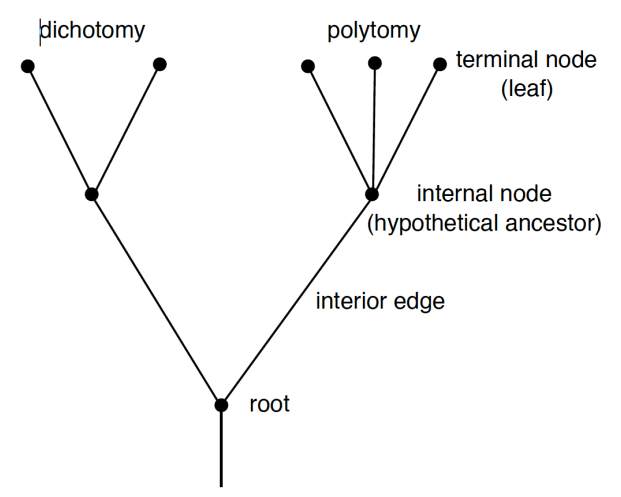
\includegraphics[width=0.3\linewidth]{figs/dichotomy-polytomy.png}
\caption{Diferencia entre dicotomía y politomía.}
\end{figure}

Los árboles filogenéticos se consideran resueltos cuando de un nodo interno salen las distintas terminales. En la mayoría de casos, los árboles son no resueltos y tienen politomías, es decir, que desde un nodo interno no se sabe cómo han avanzado las especies. A partir de ahí solo se pueden añadir más datos, pintar uniones con un bootstrap bajo (es decir, un bajo soporte de esa bifurcación), o justificar que estamos atestiguando un momento de especiación. Dentro de las hipótesis filogenéticas siempre hay más de una solución (se producen varios árboles igualmente óptimos), así que el árbol final se debe elegir. Un árbol de consenso puede ser construido mostrando las porciones de bifurcación resueltas comúnmente y colapsando aquellas que no concuerdan entre los árboles. En un árbol de consenso estricto, todos los nodos en conflicto son colapsados.

\begin{figure}[htbp]
\centering
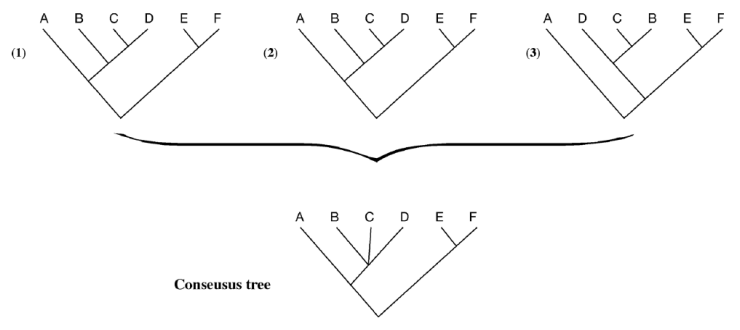
\includegraphics[width=0.5\linewidth]{figs/consensus-tree.png}
\caption{Árbol de consenso.}
\end{figure}

\section{Tipos de árboles filogenéticos}
Existen distintos tipos de árboles filogenéticos. Los \textbf{filogramas (phylogram}) miden en las ramas los cambios que ha habido por sitio, por lo que las longitudes de las ramas representan a escala la cantidad de divergencia evolutiva. Tienen la ventaja de mostrar tanto las relaciones evolutivas como la información sobre el tiempo relativo de divergencia de las ramas. Los \textbf{cladogramas (cladogram)} muestran la similitud de los distintos elementos, pero las longitudes de sus ramas no son proporcionales al número de cambios evolutivos y, por tanto, no tienen ningún significado filogenético. Los \textbf{cronogramas (chronogram)} representan la relación de los elementos de forma temporal.

\begin{table}[h]
\centering
\begin{tabular}{l c c}
\hline
\multicolumn{1}{l}{[phyl(o) gr. 'raza', 'estirpe']} & \multirow{3}{1em}{+} & \multirow{3}{12em}{[-gram-ma gr. 'representación gráfica']} \\
\multicolumn{1}{l}{[klad(o) gr. 'rama']} & & \\
\multicolumn{1}{l}{[khron(o) gr. 'tiempo']} & & \\
\hline
\end{tabular}
\caption{Tabla con términos griegos y sus significados.}
\end{table}

\begin{figure}[htbp]
\centering
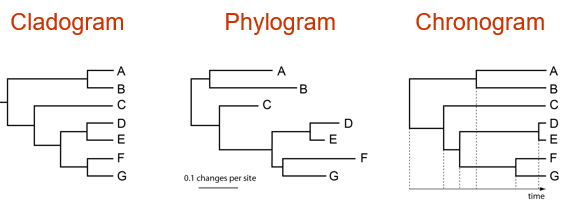
\includegraphics[width=0.5\linewidth]{figs/tipos-arboles.png}
\caption{Tipos de árboles filogenéticos.}
\end{figure}

\section{Inferencia filogenética}
Cualquier episodio histórico es, por definición, irrecuperable. La única forma que tenemos de reconstruirlo es a través del estudio de sus efectos. Por ello, la reconstrucción filogenética es un proceso de inferencia: se intenta obtener la mejor estimación posible de una historia evolutiva basada en la información incompleta y con frecuencia ruidosa contenida en los datos. Las evidencias que se emplean se basan en la morfología (comparación entre caracteres de especies), la ultraestructura (cortes vistos al microscopio electrónico), embriología (fases del desarrollo embrionario), la paleontología (registro fósil), la etología (comportamiento animal -> para estudiar evolución simpátrica), la bioquímica y las moléculas. 

Un \textbf{carácter} es una característica de los taxones que, en principio, es heredada (si no es heredada, no se puede utilizar la filogenia). El \textbf{estado de carácter} es el valor específico que toma un carácter en un taxón concreto. Por ejemplo, un carácter sería tener ojos y el estado de ese carácter sería 2 para humanos y 8 para algunas arañas.

\section{Homología}
La \textbf{homología} es la relación que existe entre dos partes orgánicas diferentes de dos organismos distintos cuando sus determinantes genéticos tienen el mismo origen evolutivo, es decir, cuando un mismo órgano tiene diversas formas y funciones. Los caracteres que se estudian en filogenia deben ser homólogos. Se compara la semejanza de una estructura debido a la herencia común. Por el contrario, la analogía es una estructura semejante a otra o que tiene la misma función, pero cuyo desarrollo embrionario y origen son diferentes. No se presentan en un antepasado común (como en el caso de los caracteres homólogos), si no que es fruto de convergencia evolutiva.

En genética y biología molecular, también existe homología en las secuencias. Se distinguen dos tipos: la ortología y la paralogía. Los \textbf{genes ortólogos} son semejantes por pertenecer a dos especies que tienen un antepasado común. Los \textbf{genes parálogos} son aquellos que se encuentran en el mismo organismo y cuya semejanza revela que uno procede de la duplicación del otro (y puede adquirir funciones diferentes del gen original). La ortología requiere que se haya producido especiación, mientras que esta no es necesaria en el caso de la paralogía, que puede producirse solo en los individuos de una misma especie. Por ello, idealmente se deben comparar caracteres ortólogos para hacer las reconstrucciones filogenéticas.

\begin{figure}[htbp]
\centering
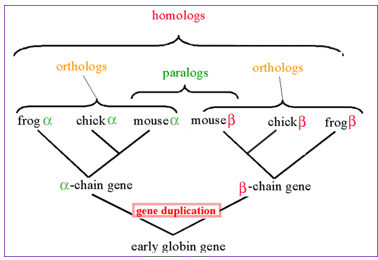
\includegraphics[width=0.5\linewidth]{figs/ortologos-paralogos.png}
\caption{Homología en genes de la hemoglobina.}
\end{figure}

%11/09 - Patricia Álvarez
\subsection{Tipos de homología}
En cladística, se emplean unas clasificaciones de las propiedades de organismos basándose en similitudes derivadas. Una \textbf{plesiomorfía} se refiere al estado \textit{ancestral} (o \textit{primitivo}) de un carácter que comparten distintas especies por heredarlo del antepasado común; en el árbol filogenético de ejemplo se presenta en los ancestros y los grupos externos. En contraposición, la \textbf{apomorfía} es un carácter novedoso evolutivamente y se dice que es \textit{derivado}, ya que deriva de otro rasgo perteneciente a un taxón ancestral filogenéticamente próximo. Así, se emplean los adjetivos plesiomófico y apomórfico en lugar de primitivo y avanzado para evitar juicios de valor sobre la evolución de los carácteres. 
Además, una \textbf{sinapomorfía} es una apomorfía (carácter exclusivo) compartida por un ancestro común y todos sus descendientes; y una \textbf{simplesiomorfía} se refiere a una plesiomorfía (carácter ancestral) compartida por dos o más taxa. Finalmente, una \textbf{autapomorfía} es un carácter novedoso y único de un taxón que no aparece en el antepasado, por lo que no lo comparte con ningún otro. 

\begin{table}[htbp]
\begin{mdframed}[backgroundcolor=black!10]
    \centering
    El prefijo "sin" viene de "compartido". Por tanto, los caracteres sinapomorfos son caracteres apomorfos compartidos, mientras que las simplesiomorfías son plesiomorfías compartidas.
    \end{mdframed}
\end{table}

\begin{table}[h]
\centering
\begin{tabular}{l c c }
\hline
\multicolumn{1}{l}{[sýn- gr. 'con', 'unión']} & \multirow{4}{*}{+} & \multirow{2}{*}{[morph gr. 'forma']} \\
\multicolumn{1}{l}{[plēsio- gr. 'cercano']} & &  \\
\multicolumn{1}{l}{[aut(o)- gr. 'que actúa por sí mismo']} & & \multirow{2}{*}{[-íā gr. 'cualidad']}  \\
\multicolumn{1}{l}{[apó- gr. 'a partir de' (derivado, novedoso)]} & & \\
\hline
\end{tabular}
\caption{Tabla con términos griegos y sus significados.}
\end{table}

\begin{figure}[htbp]
\centering
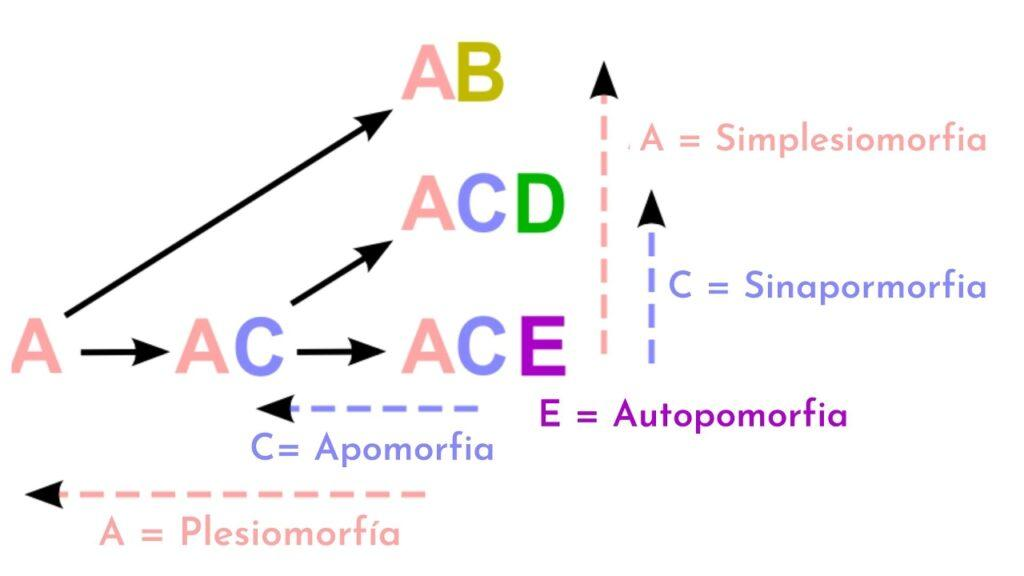
\includegraphics[width=0.5\linewidth]{figs/sinapomorfia.jpg}
\caption{Tipos de homología en el árbol filogenético (tumbado). El carácter A es plesiomórfico al estar en el ancestro. El carácter C es apomórfico al ser una novedad evolutiva. En los nodos terminales, el carácter A se considera simplesiomórfico al estar compartido por los descendientes y ser un carácter ancestral. Por el contrario, el carácter C en los nodos terminales es sinapomórfico por ser un carácter novedoso y estar compartido en el ancestro en el que surgió y sus descendientes. Los caracteres B, D y E son autopomorfos por estar presentes en un único nodo terminal.}
\end{figure}

\subsection{Homoplasia}
La homoplasia es el cambio evolutivo paralelo que hace que dos organismos presenten un mismo carácter adquirido independientemente. La \textbf{convergencia} se da cuando dos estructuras similares han evolucionado independientemente a partir de estructuras ancestrales distintas y por procesos de desarrollo diferentes. Se considera que el \textbf{paralelismo} involucra patrones de desarrollo similares en líneas evolutivas diferentes, pero próximas. La diferencia con la convergencia es que en el paralelismo, hay un ancestro que no presenta un carácter y dos descendientes directos sí presentan esa novedad evolutiva, mientras que en la convergencia los descendientes con carácter no tienen el mismo ancestro común directo. No obstante, en la práctica, la distinción entre convergencia y paralelismo es un tanto arbitraria porque no existe una regla exacta para limitar la antigüedad del antepasado común. Finalmente, en la \textbf{reversión}, un organismo adquiere un carácter de sus antepasados más lejanos. Esto implica que uno o más caracteres adquiridos previamente se han eliminado y se han vuelto a los más anteriores. 

\begin{figure}[htbp]
\centering
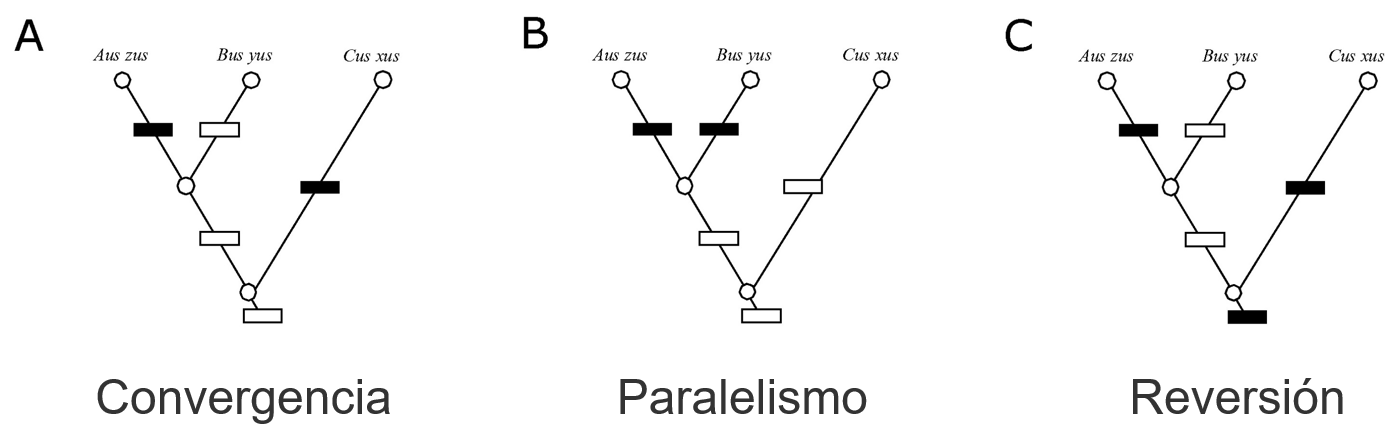
\includegraphics[width=0.5\linewidth]{figs/homoplasia.png}
\caption{Diferencias entre convergencia, paralelismo y reversión.}
\end{figure}

\subsection{Agrupamientos}
Un \textbf{grupo monofilético} es un clado que contiene un ancestro y todos sus descendientes, formando así un solo grupo evolutivo. Un \textbf{grupo parafilético} es similar, pero excluye a algunos de los descendientes que han sufrido cambios significativos. Un grupo con miembros de líneas evolutivas separadas se llama \textbf{polifilético}, conteniendo así grupos de especies con distintos ancestros comunes. 

\begin{figure}[htbp]
\centering
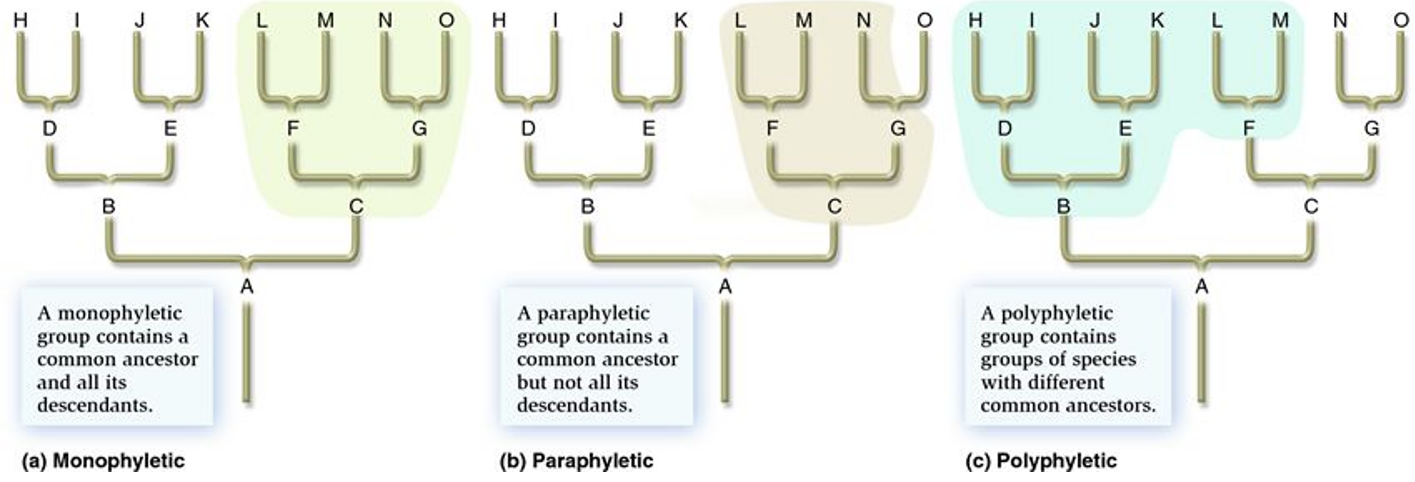
\includegraphics[width=0.5\linewidth]{figs/agrupamientos.png}
\caption{Agrupamientos de grupos monofiléticos, parafiléticos y polifiléticos.}
\end{figure}

De esa forma, los grupos monofiléticos presentan sinapomorfía, los grupos parafiléticos presentan simplesiomorfía, y los grupos polifiléticos homoplasia. 

\begin{figure}[htbp]
\centering
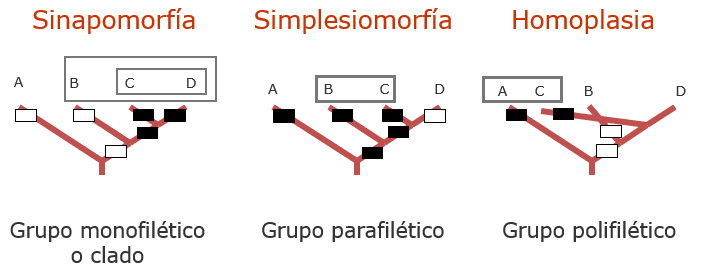
\includegraphics[width=0.5\linewidth]{figs/homoplasia-agrupamientos.png}
\caption{Grupos y caracteres que se apoyan.}
\end{figure}

\subsection{Fenotipo vs moléculas}
Tradicionalmente se han empleado los \textbf{carácteres fenotípicos} para establecer las relaciones filogenéticas. Esto se debe a que suelen ser carácteres evolutivamente relevantes y complejos menos proclives a la homoplasia. Además, son los únicos carácteres disponibles en algunos casos como en fósiles o especímenes raros. No obstante, puede haber problemas de codificación de taxones supraespecíficos como terminales (quimera ¿¿NO??) y se pueden dar casos de subjetividad en la codificación de carácteres. Además, hay un número limitado de carácteres fenotípicos y podemos encontrar taxones altamente autapomórficos. 

Recientemente se están empleando \textbf{carácteres moleculares} al ser estrictamente heredables y no haber ambigüedades en la codificación. Por ello, determinar el estado de los carácteres es trivial. Hay ciertas regularidades en la evolución de los carácteres moleculares, y éstos son robustos frente a la distancia evolutiva. También son muy abundantes y ofrecen información temporal. El problema de los carácteres moleculares es que son más proclives a la homoplasia al tener solo 4 nucleótidos y 20 aminoácidos. La evolución de estos carácteres es compleja. Además, los árboles de genes no siempre coinciden con los árboles de especies. La determinación de la homología puede ser difícil por duplicación o pérdida de genes y alineamientos. 

Se suelen utilizar multitud de genes separados y analizarlos de forma separada. El consenso de análisis separados es una estimación conservadora de la filogenia. Algunos métodos filogenéticos sólo se pueden aplicar a ciertos tipos de datos. A nivel de especies, la concatenación de genes diferentes puede ser inapropiada si se da transferencia horizontal de genes, hibridación, duplicación de genes o coalescencia más profunda que el tiempo de divergencia. El conflicto entre caracteres se resuelve teniendo en cuenta toda la evidencia disponible y realizando análisis combinados. Diferentes tipos de datos proporcionan información a diferentes niveles filogenéticos. La señal filogenética aumenta debido a la congruencia entre caracteres de diferentes conjuntos de datos. 

Es importante que el conjunto de datos sea lo más completo posible. Es necesario hacer un muestreo de taxones (incluyendo los grupos externos) y genes razonable y justificado. 

%11/09 - Patricia Álvarez
\chapter{Alineamiento de secuencias}
Decidir qué caracteres investigar, y cómo codificarlos, es un primer paso crucial en cualquier análisis filogenético. 

\section{Tipos de caracteres}
Hay \textbf{sitios invariables} que no cambian en los distintos taxones. También hay \textbf{sitios filogenéticamente neutrales} que son autapomorfías. Los \textbf{sitios filogenéticamente informativos} son comunes por pares, por lo que son sinapomorfías. 

\begin{figure}[htbp]
\centering
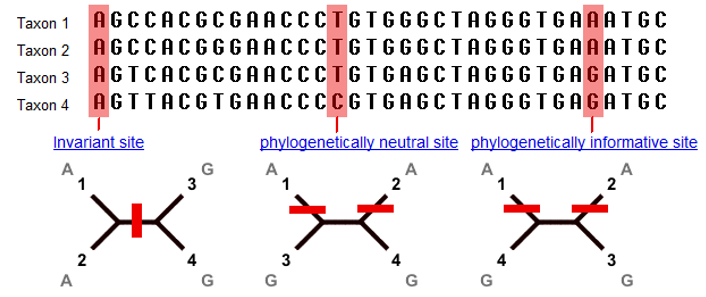
\includegraphics[width=0.5\linewidth]{figs/sitios-informativos.png}
\caption{Sitios en una secuencia invariantes (no cambian entre los distintos taxones), filogenéticamente neutrales (solo cambia en un taxón) y filogenéticamente informativos (permiten dicotomía).}
\end{figure}

Los caracteres pueden ser \textbf{binarios 0/1} (presentes o ausentes), \textbf{multiestado} o \textbf{binarios V/S} (transversiones o transiciones). Los caracteres también pueden ser \textbf{discretos o continuos}. La codificación de caracteres continuos no se pueden incluir fácilmente en las matrices de caracteres, por lo que se debe realizar una categorización arbitraria. Idealmente, se deben buscar divisiones naturales, es decir, estados discretos de un carácter de variación continua. 

\section{Ponderación de los caracteres}
Se puede emplear un valor relativo de los diferentes caracteres y transformaciones como indicadores de las relaciones filogenéticas entre taxones. Se puede realizar una ponderación uniforme, que minimiza los supuestos del análisis, o una ponderación diferencial, en la que no todas las características de un organismo tienen el mismo valor como evidencias filogenéticas. 

\subsection{Ponderación \textit{a priori}}
En la ponderación \textit{a priori} de caracteres morfológicos, los taxónomos pueden tener muchas razones para asumir que diferentes caracteres tienen diferente importancia filogenética. Pero eso tiene dos problemas: diferentes opiniones expertas y, en caso de acuerdo, el peso proporcional que se le da a cada carácter. Se introduce precisamente el tipo de subjetividad que el análisis cladístico pretende evitar.

\subsection{Ponderación \textit{a posteriori}}
El método más utilizado y aplicado, denominado \textbf{ponderación implícita}, se basa en Goloboff (1993): la primera vez que un carácter cambia de estado en un árbol, este cambio de estado recibe el peso «1»; los cambios posteriores son menos «costosos» y reciben pesos menores a medida que la tendencia de los caracteres a la homoplasia se hace más evidente. Los árboles que maximizan la función cóncava de homoplasia resuelven el conflicto de caracteres a favor de los caracteres que tienen más homología (menos homoplasia) e implican que el peso medio de los caracteres sea lo más alto posible.

Goloboff reconoce que los árboles con los pesos medios más elevados son los que más «respetan» los datos: un peso medio bajo implica que la mayoría de los caracteres están siendo «ignorados» por los algoritmos de construcción de árboles. Aunque originalmente se propuso con una ponderación severa de k=3, Goloboff prefiere ahora concavidades más «suaves» (por ejemplo, k = 12), que han demostrado ser más eficaces en casos simulados y del mundo real.

$$F = \sigma fi, fi = \frac{k}{k+(s-m)} $$

siendo m el número mínimo de pasos, s el número de pasos observados y k la constante de concavidad.

\subsection{Secuencias de ADN}
 Generalmente, se toma la tasa de sustitución como medida de la fiabilidad de la información filogenética del marcador. Se entiende entonces homoplasia como saturación. Las transversiones evolucionan lentamente y aumentan su frecuencia a medida que pasa el tiempo. Las transiciones se saturan a partir de cierta distancia filogenética, perdiéndose su señal. 
 
El coste de las transformaciones se determina empíricamente mediante matrices de costes (stepmatrices). 

\section{Polaridad de los caracteres}
Necesitamos conocer la polaridad de los caracteres para poder enraizar los árboles. Para ello, se debe establecer qué carácter es ancestral y qué carácter es derivado. Utilizando un \textbf{criterio ontogenético}, se ve cómo se forma el carácter durante el desarrollo para poder establecer la polaridad. En caso de que no quede claro tras ese criterio, se compara con el outgroup para establecer el estado primitivo del carácter. 

\section{Homología de los caracteres moleculares}
Cuando analizamos secuencias, asumimos que son de moléculas heredadas de ancestros a descendientes (ortólogos). Cada secuencia está formada por muchos caracteres (cada posición en la secuencia). Por ello, un primer paso es determinar el estado de cada uno de esos caracteres en cada taxón de la matriz. Importante: La homología de los caracteres moleculares, como la de cualquier otro tipo de carácter, es un concepto cualitativo. Las secuencias del gen A de dos taxones son homólogas, o bien no lo son. Igualmente, la posición X en la secuencia de un taxón es homóloga de la posición Y en la secuencia de otro taxón, o bien no lo es. Pero NO puede decirse que las secuencias de dos taxones muestren mayor o menor homología (por ejemplo, en \%). Podrán tener diferente porcentaje de similitud (p. ej., \% de bases o aminoácidos idénticos en posiciones homólogas), pero o son homólogas o no lo son.

\subsection{Aplicación del concepto de homología a los genes: alineamiento de secuencias}
Un alineamiento es una hipótesis acerca de la homología posicional de diferentes secuencias de bases o aminoácidos. El alineamiento tiene como objetivo identificar qué posiciones son homólogas en diferentes secuencias. Cada posición de la secuencia (residuo = nucleótido o aminoácido) se interpreta como un carácter que puede tomar diferentes valores (estados de carácter: una de 4 bases, o uno de 20 aminoácidos). El alineamiento asume parsimonia: el cambio evolutivo es improbable, de modo que los segmentos de secuencia coincidentes sirven de guía para identificar posiciones homólogas. Eventualmente se identifican cambios, que cuando son compartidos por varias especies son informativos para la reconstrucción de filogenias.

Las secuencias pueden no tener la misma longitud. Los gaps son marcadores de posición que introducimos en los alineamientos para mantener la homología posicional. Representan eventos de inserción o pérdida denominados indels (del inglés insertion/deletion). La ventaja es que los indels son, en principio, menos propensos a la homoplasia que las sustituciones de bases, muy utilizadas en análisis de parsimonia. No obstante, los indels son difícilmente gestionables por la mayoría de los modelos de evolución molecular. 

Es importante elegir un buen alineamiento, ya que la calidad del alineamiento influye en la calidad de la inferencia filogenética. 

%\subsection{Alineamientos globales vs locales} -> se lo saltó
%En el \textbf{alineamiento global}, se intenta alinear cada residuo en cada secuencia. Son especialmente útiles para alinear secuencias emparentadas de tamaño similar (las que se usan para la reconstrucción filogenética). El \textbf{alineamiento local} se utiliza para secuencias poco parecidas que se supone que contienen regiones similares, o para identificar la ubicación de motivos concretos en contextos más amplios (por ejemplo, BLAST). 

\subsection{Decidir el mejor alineamiento}
No existe ningún procedimiento automático para elegir objetivamente el mejor alineamiento: hay que valorar la calidad de los diferentes alineamientos posibles y elegir el que nos parezca mejor. Elegimos como mejor alineamiento el supuesto más razonable de acuerdo con un algoritmo informático y el ojo experimentado. En cualquier caso, es siempre importante examinar el resultado críticamente para valorar si tiene sentido desde un punto de vista biológico.

No todos los alineamientos son igualmente parsimoniosos. Para valorar la calidad de los alineamientos, se han propuesto diferentes mecanismos de puntuación. Se puede realizar una \textbf{puntuación por identidad}. Un alineamiento de dos secuencias puede interpretarse como una matriz con dos filas y n columnas (n = longitud del alineamiento). Las posiciones (columnas) con idéntico residuo (base o aminoácido) tienen una puntuación = 1. La puntuación del alineamiento es la suma de las puntuaciones de todas sus posiciones. El alineamiento óptimo es el que maximiza la identidad de las columnas. No obstante, los gaps no penalizan, por lo que pueden darse alineamientos con misma puntuación, pero más posiciones de diferencia. Por tanto, se pueden aplicar penalizaciones para los huecos en la secuencia, ya sea introduciendo penalizaciones por la apertura de los huecos o por la extensión de los huecos abiertos. Estos últimos son típicamente menores que las impuestas por apertura. Por ejemplo, se puede aplicar una penalización de -2 por apertura de gap y de -1 por extensión del gap abierto.  

\begin{figure}[htbp]
\centering
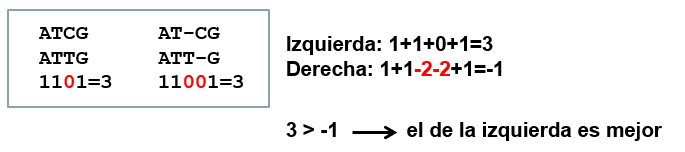
\includegraphics[width=0.5\linewidth]{figs/mejor-alineamiento.png}
\caption{Ejemplo de cálculo del mejor alineamiento.}
\end{figure}

No tiene mucho sentido alinear las secuencias de ADN de los genes codificantes de proteínas. Es mejor traducir las secuencias de ADN a secuencias de aminoácidos y alinear éstas últimas. Existen varios programas para alineamiento múltiple: clustal W/X/Omega, MAFFT, Muscle, T-Coffee, Dialign 2, etc. 

%Nos saltamos la diapositiva 42 y de la 44 a la última.



%11/09 - Patricia Álvarez
\chapter{Modelos de evolución}
Todos los métodos de inferencia y reconstrucción filogenética implican una serie de \textbf{supuestos}, aunque éstos no se hagan explícitos: \begin{itemize}
\item Todos los sitios o posiciones cambian independientemente. 
\item Las tasas de evolución son constantes a lo largo del tiempo y entre linajes.
\item La composición de bases es homogénea.
\item La verosimilitud de los cambios de base es la misma para todos los sitios y no cambia a lo largo del tiempo. 
\end{itemize}

Esto son asunciones, pero en realizar no son ciertos. Las tasas de evolución no son constantes, las posiciones no cambian independientes las unas de las otras, la composición de bases no es homogénea (hay mayor porcentaje de GC que de AT) y se pueden dar múltiples cambios en un único sitio que quedan ocultos (si el nucleótido original es C, puede que en un organismo cambie a A y en otro a G). Estos cambios ocultos hacen que las secuencias estén cada vez más saturadas: la mayoría de los sitios que cambian han cambiado antes. 

En un contexto filogenético, los modelos predicen el proceso de sustitución de las secuencias a través de las ramas. Describen probabilísticamente el proceso por el que los estados de los caracteres homólogos de las secuencias (posiciones alineadas: nucleótidos o aminoácidos) cambian a lo largo del tiempo.

Los modelos implican por lo general los siguientes \textbf{parámetros}: \begin{itemize}
\item \textbf{Composición:} frecuencia de las diferentes bases o aminoácidos.
\item \textbf{Proceso de sustitución:} tasa de cambio de uno a otro estado de carácter.
\item \textbf{Otros parámetros (heterogeneidad de tasas):} proporción de sitios invariables o agregación de los cambios a lo largo de la secuencia.
\end{itemize}

\section{Modelos frecuentes}
El modelo más sencillo es el de Jukes Cantor, el cual asume que todos los cambios son igualmente probables y que la frecuencia de todas las bases es la misma. A partir de este, la complejidad empezó a aumentar, ya que las combinaciones de parámetros son muchas. Algunos de los modelos más frecuentes son: \begin{itemize}
\item \textbf{Jukes and Cantor (JC69)}: La frecuencia de todas las bases es la misma (0.25 cada una), y la tasa de cambio de una a otra base es igual.
\item \textbf{Kimura 2-parámetros (K2P)}: La frecuencia de todas las bases es la misma (0.25 cada una), pero la tasa de sustitución es diferente para transiciones y transversiones.
\item \textbf{Hasegawa-Kishino-Yano (HKY)}: Como K2P, pero la composición de bases varía libremente.
\item \textbf{General Time Reversible (GTR)}: La composición de bases varía libremente, y todas las sustituciones posibles pueden tener distintas frecuencias.
\end{itemize}

Cada vez, los modelos son más complejos, y normalmente se utiliza el más complejo. Hay programas que ya proponen un modelo a elegir según los datos que se le proporcionen. 
%16/09 - Patricia Álvarez
\chapter{Métodos filogenéticos de inferencia}
Los pasos generales en el proceso de reconstrucción filogenética son: \begin{enumerate}
\item Diseño experimental: selección del ingroup y outgroup, selección de los marcadores moleculares
\item Recolección de datos de secuencia homóloga
\item Ensamblaje de la matriz de secuencias
\item Alineamiento de la secuencia
\item Selección del modelo
\item Inferencia filogenética
\item Construcción del árbol filogenético: soporte estadístico, testar hipótesis filogenética, estimación del tiempo de divergencia
\end{enumerate}

\section{Búsqueda de árboles}
Sólo hay una manera de construir el primer  árbol sin raíz, uno con tres puntas (nodos terminales) y tres ramas. Cada vez que añadimos un taxón, se crean dos ramas. Un árbol con n puntas (taxones) tendrá por tanto 2n-3 ramas.

A partir de unas pocas especies, las búsquedas de árboles sin raíz son exhaustivas y computacionalmente demasiado exigentes. Por ello, se realiza una \textbf{búsqueda heurística}: 
\begin{enumerate}
\item Construir el árbol inicial (Ej., mediante adición secuencial de taxones) y determinar su longitud (ver el número de cambios de un taxón a otro).
\item Construir un conjunto de “árboles vecinos” o alternativos haciendo pequeñas reordenaciones en el árbol inicial, y determinar las longitudes de cada nuevo árbol.
\item Si cualquiera de los árboles vecinos es mejor que el inicial (tienen un menor número de pasos o cambios evolutivos, es decir, la hipótesis se ajusta mejor a los datos): retenerlo y usarlo como punto de partida para una nueva ronda de reordenaciones (es posible que varios de estos árboles sean igual de buenos).
\item Repetir pasos 2 y 3 hasta encontrar un árbol que es mejor que todos sus vecinos.
\item Este árbol es un óptimo local (¡no necesariamente un óptimo global!)
\end{enumerate}

El procedimiento semeja un paseo en un paisaje montañoso, donde nos interesa alcanzar la cumbre más alta (hill climbing).

\begin{figure}[htbp]
\centering
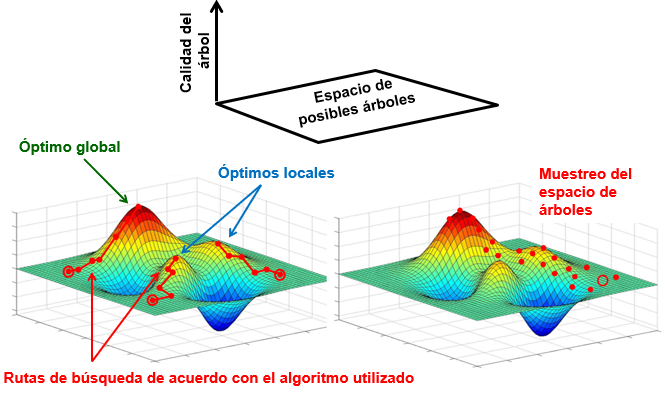
\includegraphics[width=0.7\linewidth]{figs/busqueda-heuristica.png}
\caption{Búsqueda heurística del mejor árbol.}
\end{figure}

Hay varios \textbf{algoritmos de reordenación de ramas (branch swapping)}: \begin{itemize}
\item \textbf{Nearest Neighbour Interchange (NNI):} intercambia dos vecinos por cada rama interna.
\item \textbf{Subtree Pruning and Regrafting (SPR):} se corta un clado (subárbol) y se empalma en todas las ramas del resto del árbol, usando el punto de corte del subárbol como punto de unión. Realmente, NNI es un subconjunto de SPR. 
\item \textbf{Tree Bisection and Reconnection (TBR):} se divide el árbol en dos partes y se reconectan los subárboles usando todos los posibles pares de ramas. NNI y SPR son subsets de TBR.
\end{itemize}

\begin{figure}[htbp]
\centering
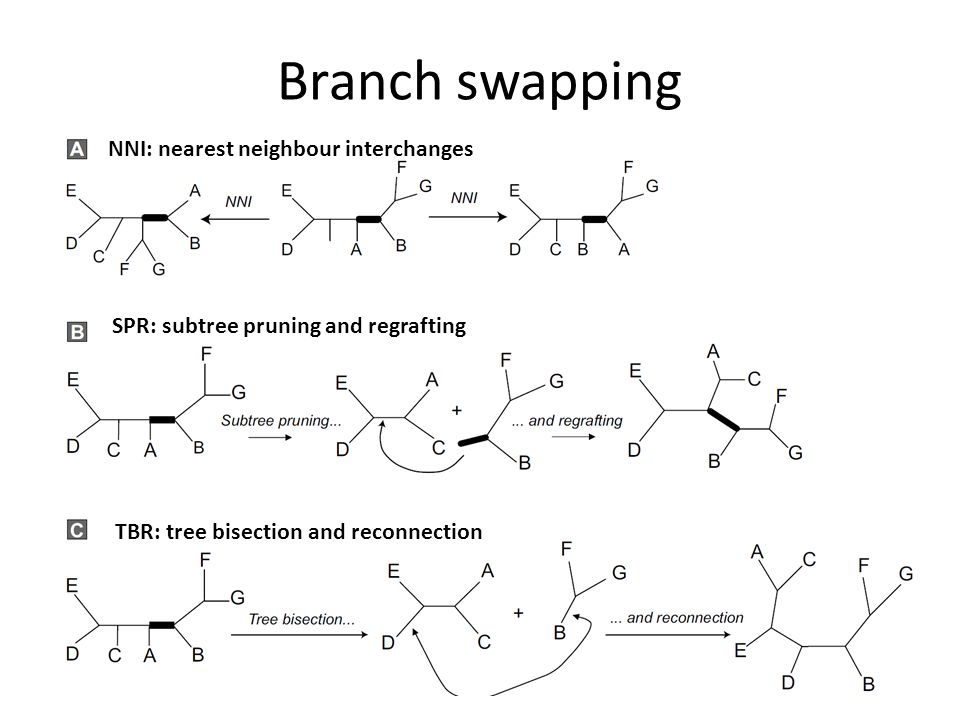
\includegraphics[width=0.7\linewidth]{figs/branch-swapping.jpg}
\caption{Esquemas de los distintos algoritmos de reordenación de ramas.}
\end{figure}

El espacio de árboles puede estar poblado por mínimos locales e islas de árboles óptimos.

\begin{figure}[htbp]
\centering
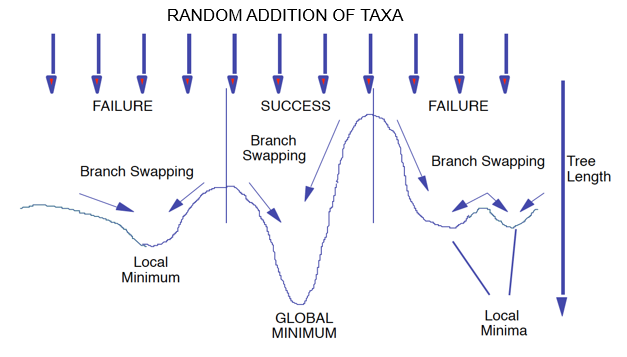
\includegraphics[width=0.7\linewidth]{figs/result-swapping.png}
\caption{Posibles resultados de árboles tras la adición de taxones.}
\end{figure}

\section{Árboles de consenso}
A menudo existen varios árboles candidatos a ser el cladograma más parsimonioso\footnote{véase explicación de parsimonia en el tema 5}. En el siguiente ejemplo, hay tres cladogramas diferentes que son igualmente parsimoniosos para los 4 caracteres estudiados (1-4) en cuatro especies de homínidos. Si aumentamos el número de caracteres y el de taxones, la cantidad de cladogramas igualmente parsimoniosos se dispara y se hace inmanejable. Por lo tanto, es conveniente contar con formas estandarizados de resumir los puntos de acuerdo entre cladogramas rivales para llegar a formar un “árbol de consenso”.

\begin{figure}[htbp]
\centering
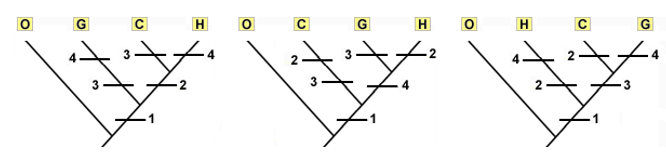
\includegraphics[width=0.7\linewidth]{figs/cladogramas-hominidos.png}
\caption{Tres cladogramas igualmente parsimoniosos de cuatro especies de homínidos: orangutanes, gorilas, chimpancés y humanos.}
\end{figure}

Un árbol de consenso no es otra cosa que un árbol que combina los agrupamientos preferidos a partir de los cladogramas rivales de un determinado grupo de taxones, de tal forma que los agrupamientos discutibles (contenciosos, ambiguos) se condensan en puntos con múltiples ramas (politomías= nodos que portan múltiples ramas). Existen diferentes formas para construir árboles de consenso, pero los tres métodos más comunes son: \begin{itemize}
\item \textbf{Árbol de consenso estricto:} conserva sólo los agrupamientos que comparten todos los cladogramas rivales.
\item \textbf{Árbol de consenso semi-estricto o loose:} conserva todos los agrupamientos que no son contradictorios en los cladogramas rivales.
\item \textbf{Árbol de consenso de regla de la mayoría:} conserva todos los agrupamientos que son apoyados por la mayoría de cladogramas rivales, aunque contradigan a la minoría. Este es el que más se utiliza.
\end{itemize}

\begin{figure}[htbp]
\centering
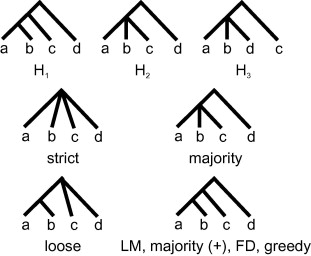
\includegraphics[width=0.5\linewidth]{figs/consensus-trees-types.jpg}
\caption{Distintos tipos de árboles de consenso.}
\end{figure}

Cuando tenemos muchos taxones entre los cuales hay mucha homoplasia, los árboles de consenso estricto van a mostrar gran número de politomías que no pueden resolverse ya que existen conflictos de agrupamiento entre los cladogramas rivales. En esos caso, los árboles de consenso basados en la regla de la mayoría, ofrecen al menos bastantes más hipótesis de trabajo para investigar las relaciones filogenéticas. El ejemplo está basado en más de 70 especies de erizos irregulares; para mayor claridad se han omitido los nombres de las especies. Se estimó que había más de 70.000 cladogramas igualmente parsimoniosos, lo que refleja un gran componente de homoplasia entre los caracteres analizados. El árbol de consenso estricto resultante, ofrece por tanto poca resolución, y la mayoría de los taxones de agrupan en una gran politomía. Por el contrario, el árbol de consenso de regla de la mayoría, resuelve un número de clados mucho mayor que podrán comprobarse en sucesivos análisis. Los valores numéricos para el árbol de consenso de regla de la mayoría miden el porcentaje de cladogramas igualmente parsimoniosos que apoyan cada grupo resuelto.

\begin{figure}[htbp]
\centering
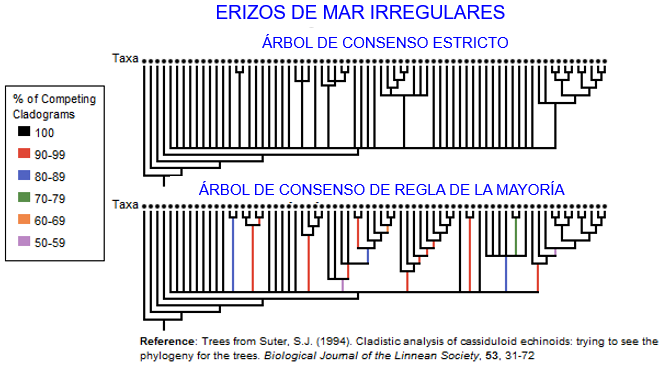
\includegraphics[width=0.7\linewidth]{figs/arbol-erizos.png}
\caption{Árboles filogenéticos de erizos de mar irregulares.}
\end{figure}

\section{Medidas de soporte: confianza en el árbol}
La mayor parte de las medidas científicas van acompañadas de una estima de su precisión del tipo. En el caso de la inferencia filogenética, no es suficiente con estimar hipótesis filogenéticas, sino que es necesario indicar una estima de la confianza que dicha hipótesis presenta. Esto se debe a: 
\begin{itemize}
\item \underline{Error de muestreo:} Nuestros análisis están basados en muestras, pero sólo tenemos una muestra de los datos. Los valores estimados a partir de muestras de una población raramente van a coincidir con el valor real. Una forma de calcular este error es tomando múltiples muestras y comparando las estimas obtenidas entre sí.
\item \underline{Error sistemático:} Asociado a la metodología y las asunciones de los análisis.
\end{itemize}

Las formas de dar apoyo y soporte a un nodo se pueden dar de forma cualitativa (soporte de Bremer), remuestreo (bootstrapping, jackknife) y probabilístico (probabilidad posterior bayesiana): 
\begin{itemize}
\item \textbf{Soporte de Bremer o Decay Index}: se calcula la diferencia en el número de pasos entre el árbol óptimo y el mejor árbol en el que no aparece el clado en cuestión.
\item \textbf{Remuestreo por bootstrapping:} se remuestrean los caracteres al azar con reemplazamiento múltiples veces. Se realiza el análisis con cada nueva pseudoréplica utilizando los mismos parámetros que en el análisis original. Se analiza la coincidencia entre las topologías obtenidas resumiéndolas en un majority-rule consensus tree. Las pseudoréplicas se construyen a partir de la matriz original con reemplazamiento para construir una nueva matriz del mismo tamaño que la original. La frecuencia con que aparece un determinado grupo es una medida de la estabilidad de ese grupo. Estos valores se muestran en un árbol de majority-rule consensus y se da información adicional en una tabla (de biparticiones). Los valores de bootstrap son conservadores; son un índice relativo del soporte estadístico de los grupos, proporcionado por los datos que se están analizando bajo un método de análisis concreto: valores altos de bootstrap nos indican la existencia de una señal filogenética “fuerte” en los datos. Estudios realizados con datos empíricos y simulaciones han indicado que un 70\% de soporte de bootstrap puede considerarse apoyo razonable para una relación determinada. No obstante, este número se puede modificar según se necesite.
\item \textbf{Remuestreo por Jackknife:} Jackknife es muy similar al bootstrap, sólo se diferencia en la estrategia de remuestreo de los caracteres. Una cierta proporción de los caracteres es eliminada al azar (por ej.: 50\%). No hay reemplazo, por lo que la matriz es más pequeña. Se analizan las pseudoréplicas y los resultados se resumen en un majority-rule consensus tree. Jackknifing y bootstrapping suelen dar resultados similares y se interpretan de forma similar. Jackknife se está utilizando cada vez menos y se está reemplazando por bootstrap al estar reduciendo los datos.
\end{itemize}

\begin{figure}[htbp]
\centering
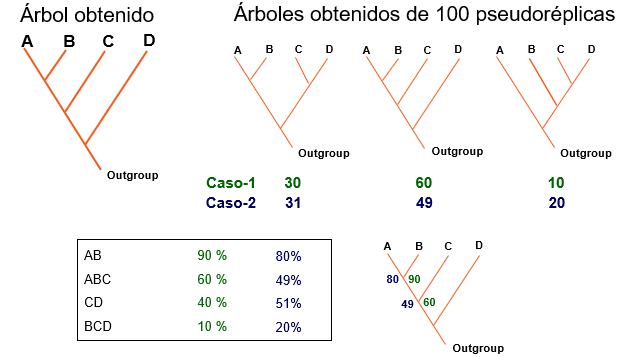
\includegraphics[width=0.7\linewidth]{figs/ejemplos-bootstrap.png}
\caption{Ejemplos del cálculo de bootstrap. En el primer caso (mostrado en verde), tras 100 pseudoréplicas, han salido tres árboles con frecuencias de 30, 60 y 10. Tanto en el primer como en el segundo árbol, los taxones A y B se han relacionado juntos, por lo que esa dicotomía tiene un soporte de bootstrap de 90 (60 + 30). La siguiente relación más soportada, con un bootstrap de 60, es la de relacionar el taxón C con el antepasado común de A y B, por lo que el árbol final muestra esa variante (la otra opción sería relacionar C con D, como hacen los otros dos árboles, pero su frecuencia es de 40). En el segundo caso (mostrado en azul), las frecuencias han cambiado. Ahora, la relación de A y B pasa a tener un soporte de 80 (31 + 49), y así sucesivamente.}
\end{figure}

%16/09 - Patricia Álvarez
\chapter{Máxima parsimonia - Cladística}
La cladística es un método de análisis de la sistemática filogenética que busca reconstruir las “genealogías” de los organismos y elaborar clasificaciones que las reflejen. Descansa sobre el axioma fundamental de que en la naturaleza, como resultado de la evolución, existe un orden que se manifiesta en las similitudes de los caracteres. Determina las relaciones evolutivas entre los organismos basándose en los caracteres relativamente derivados o apomórficos (novedades evolutivas). La reconstrucción filogenética consiste en identificar todos los grupos monofiléticos que existen en una muestra de taxones, que son aquellos definidos por sinapomorfías (caracteres derivados compartidos).

\section{Construir el árbol}
Desconocemos el aspecto del antecesor común más reciente de las especies y el modo en que están emparentadas, por lo que comenzamos a analizar sus relaciones buscando las diferentes formas en que pueden ser conectadas. Este ejemplo implica mayor similitud entre red (network) o árbol sin enraizar con ramificación dicotómica que conecta un grupo de taxones. No tiene raíz que conecte con un antecesor común; es como un mapa filogenético visto desde arriba, con el antecesor común oculto por sus descendientes. Es de ramificación dicotómica porque sólo tres ramas se juntan en cada unión o nodo; cada línea se divide siempre en dos ramas. Se pueden obtener otra red cambiando la posición de las especies. Existen tres posibles formas de unir 4 especies en una red de ramificación dicotómica. 

\begin{figure}[htbp]
\centering
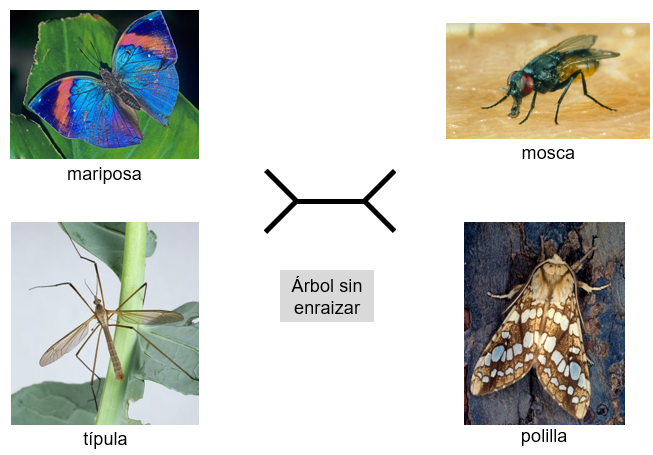
\includegraphics[width=0.5\linewidth]{figs/ejemplo-arbol-sin-enraizar.png}
\caption{Ejemplo de un árbol sin enraizar entre cuatro especies. Existen dos alternativas más árboles sin enraizar: mariposa-polilla con mosca-típula y mariposa-mosca con típula-polilla.}
\end{figure}

La selección de la explicación más sencilla de la distribución de los diferentes estados de caracteres se denomina \textbf{principio de parsimonia}. Así, se revisan los caracteres y se construye la matriz para ver cómo se sitúan los estados de los caracteres en las redes posibles. Aplicando el principio de parsimonia, se rechazan aquellos árboles que tengan más transformaciones en la red y se queda el más parsimonioso, es decir, el que necesita menos transformaciones evolutivas para explicar la distribución de los estados de los caracteres analizados. 

\begin{figure}[htbp]
\centering
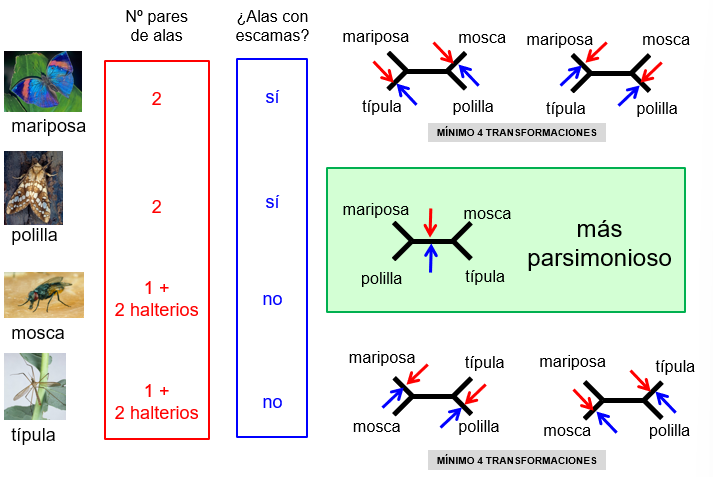
\includegraphics[width=0.5\linewidth]{figs/ejemplo-matriz-parsimonia.png}
\caption{Matriz de los estados de caracteres del ejemplo anterior. Tanto la mariposa como la polilla tienen dos pares de alas y las alas tienen escamas, mientras que la mosca y la típula tienen un par de alas y dos halterios y las alas no tienen escamas. A partir de ahí, se calculan las transformaciones necesarias para explicar la distribución del árbol y se elige el más parsimonioso, es decir, el que necesite un menor número de cambios.}
\end{figure}

Ante distintas hipótesis sobre las relaciones filogenéticas de los organismos dados, elegimos la más parsimoniosa, esto es, la que tenga una longitud menor (menor número de cambios), un mayor número de homologías y un menor número de homoplasias. Si hay varios árboles o hipótesis igualmente parsimoniosos, no podremos elegir entre ellos. La longitud de un árbol indica el número de transformaciones evolutivas necesarias para explicar los datos dada una topología de árbol concreta. Corresponde al número de cambios de estado que se producen en el árbol.

\section{Enraizar el árbol}
El siguiente paso es enraizar el árbol. La raíz nos permite determinar el lugar donde se encuentra el ancestro común. Para ello, se debe elegir la polaridad de los caracteres, es decir, conocer en qué orden se produjeron las transformaciones. Conocer qué estado del carácter es primitivo y cuál es derivado nos ayudará a elegir el cladograma con la distribución más sencilla de estados derivados (el más parsimonioso).

\begin{figure}[htbp]
\centering
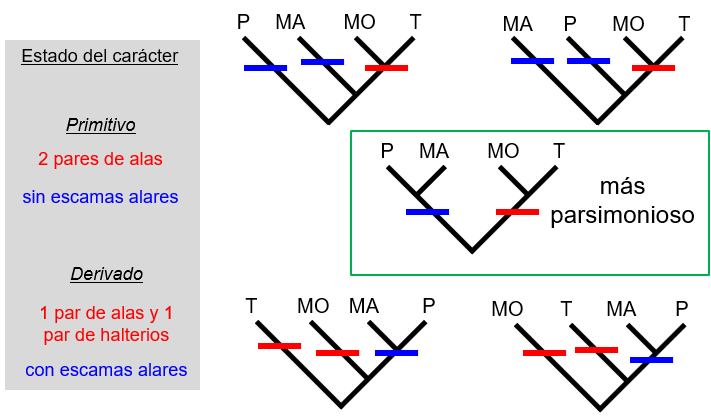
\includegraphics[width=0.5\linewidth]{figs/ejemplo-arbol-enraizado.png}
\caption{Opciones de árboles enraizados siguiendo el ejemplo anterior. Primero, sería importante conocer en qué orden se produjeron las transformaciones, si derivaron los halterios del segundo par de alas o si fue a la inversa. Supongamos que hay evidencias que sugieren que los halterios derivaron del segundo par de alas (que era el estado primitivo) y que la adquisición de escamas en las alas es otro estado de carácter derivado. En los posibles árboles, marcamos el lugar donde debe ocurrir la transformación de cada carácter de primitivo a derivado. El árbol más parsimonioso es aquel que necesita menos transformaciones para explicar la distribución de los estados derivados de los caracteres, y el que probablemente mejor registre las relaciones evolutivas de las cuatro especies de insectos.}
\end{figure}

La máxima parsimonia asume los siguientes principios: \begin{itemize}
\item \underline{Principio auxiliar de Hennig}: Ante caracteres similares y en ausencia de evidencia que indique evolución paralela o convergencia, siempre se asume que dichos caracteres son homólogos.
\item \underline{Regla de agrupación de Hennig}: Las sinapomorfías son evidencias de relaciones de ancestro común, mientras que las simplesiomorfías, las convergencias y los paralelismos no proporcionan evidencias sobre el ancestro común. 
\end{itemize}

Una auténtica homología debe circunscribir un grupo consistente con los especificados por otras homologías. Para comprobar esto, se realiza un \textbf{test de congruencia}. Así, se considera homología primaria cuando coincide, mientras que cuando se debe reinterpretar un carácter, se considera homología secundaria.

\begin{figure}[htbp]
\centering
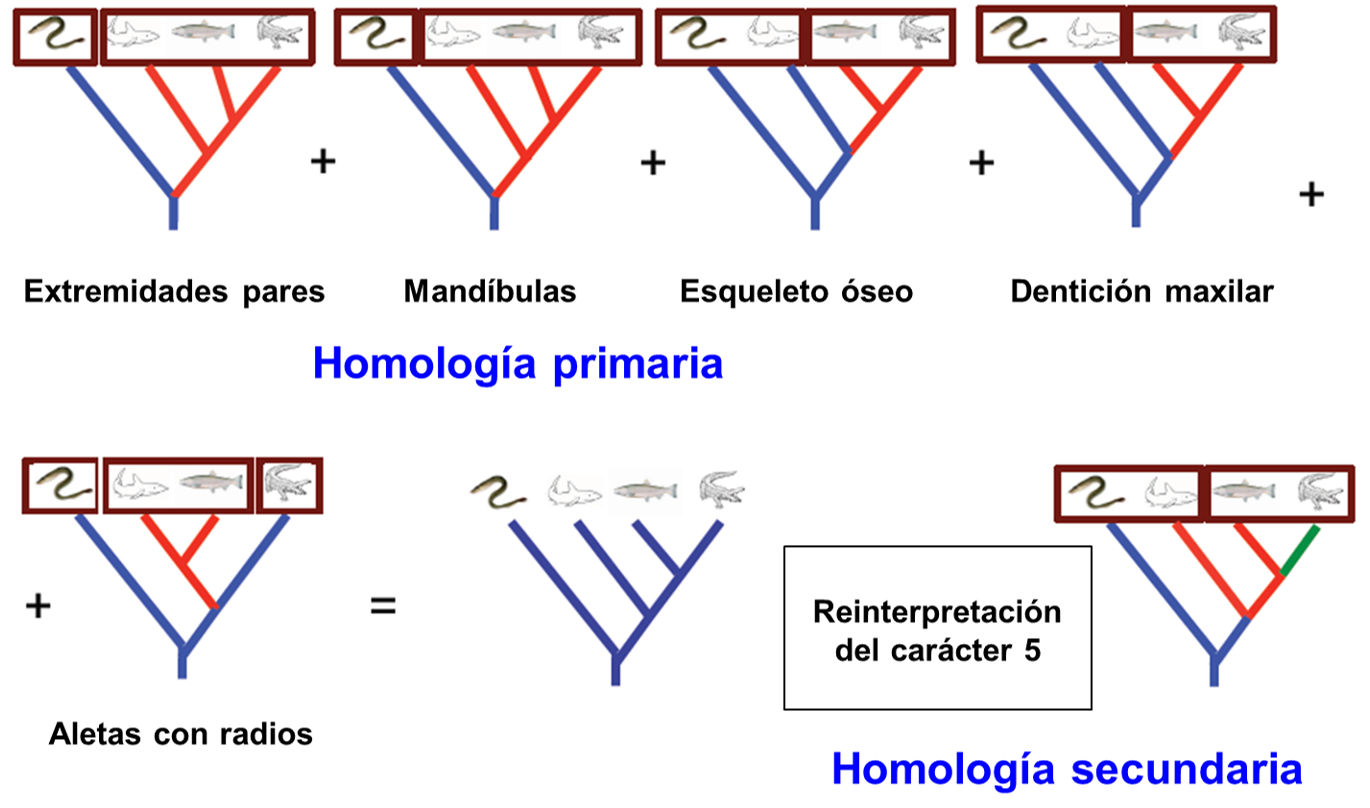
\includegraphics[width=0.5\linewidth]{figs/homologia-primaria-secundaria.png}
\caption{Árboles filogenéticos entre anguilas, tiburones, peces y cocodrilos basados en los caracteres de extremidades pares, mandíbulas, esqueleto óseo, dentición maxilar y aletas con radios. La mayoría de los árboles muestran una distribución similar de los taxones, mostrando así homología primaria. No obstante, el carácter aletas con radios es diferente, al relacionar dos taxones que en los demás caracteres no estaban relacionados. Ese carácter se debe reinterpretar, siendo así homología secundaria.}
\end{figure}

En el cladismo, se busca maximizar la congruencia entre caracteres, y así minimizar la incongruencia (homoplasia). En una aplicación computacional de la máxima parsimonia, se sigue un criterio de optimización (criterio para escoger entre diferentes cladogramas / relaciones filogenéticas), en el cual el cladograma preferido es aquél que tiene el menor número de transformaciones entre estados de carácter (pasos). Determinar los estados ancestrales implica poder identificar cambios de estado de carácter.


% \section{Valoración de árboles} -> se lo saltó
%Encontrar el cladograma más parsimonioso es la meta final de los análisis filogenéticos, aunque preguntas sobre su fiabilidad pueden permanecer. Para comparar objetivamente diferentes cladogramas y valorar el ajuste de los caracteres se han desarrollado medidas para cuantificar el alcance del problema de la homoplasia en los cladogramas obtenidos. Se comentan tres medidas: \begin{itemize}
%\item Longitud del árbol: mide el número mínimo de transformaciones que se requieren en un determinado cladograma a partir de la matriz de caracteres (los árboles de longitud mínima para una matriz se llaman árboles de Wagner).
%\item Índice de consistencia (CI): muestra la proporción de transformaciones que no se repiten (es decir, que no son homoplasias) en un cladograma.
%\item Índice de retención (RI): estima el alcance de las sinapomorfías entre los estados de los caracteres en un cladograma determinado.
%\item Índice de retención re-escalado (RCI): combina los dos anteriores, situando la homoplasia observada en una escala desde la mínima (0) a la máxima posible (1).
%\end{itemize}

%18/09 - Patricia Álvarez
\chapter{Máxima verosimilitud (ML)}
Los métodos probabilísticos se apoyan en la verosimilitud de obtener los datos (un alineamiento múltiple de secuencias) si los linajes hubieran evolucionado de acuerdo con un determinado árbol filogenético (con su topología y longitudes de las ramas) y bajo un determinado modelo de evolución molecular. La máxima verosimilitud intenta responder a la siguiente pregunta: ¿cuál es la probabilidad de observar los datos (el alineamiento), dada una hipótesis (un árbol y un modelo concreto de evolución molecular)? El árbol que hace que los datos sean el resultado más probable es una estimación de máxima verosimilitud de la filogenia. Se hacen dos estimaciones:
\begin{itemize}
\item ¿Cuál de los posibles topologías hace los datos más verosímiles? (NNI, SPR, TBR)
\item Para una topología: ¿qué longitudes de ramas hacen los datos mas verosímiles?
\end{itemize}

La verosimilitud calculada no es la probabilidad de que el árbol sea el correcto, sino lo es de que el árbol estimado generase los datos (si cambian los datos, cambia el árbol). La verosimilitud de un modelo (un árbol filogenético) es igual a la probabilidad de los datos (un alineamiento de secuencias) dada una hipótesis, es decir, un árbol y un modelo de evolución molecular. Esto es una consideración filosófica, ya que la ecuación de verosimilitud no es la probabilidad de que la hipótesis sea correcta en términos absolutos, sino para nuestros datos. La máxima verosimilitud cuenta con una serie de supuestos:
\begin{itemize}
\item Los sitios evolucionan independientemente.
\item Los cambios siguen un modelo de Markov: la probabilidad de que tenga lugar un cambio en un sitio no depende de la historia previa de ese sitio.
\item Los cambios son reversibles en el tiempo.
\end{itemize}

El procedimiento interno calcula la verosimilitud de un alineamiento de dos secuencias, dada una matriz de sustituciones, cierta composición de bases y una longitud concreta para la rama que separa esas secuencias (CED: certain evolutionary distance). Para ello, se calculan todos los eventos posibles. En caso de que haya diferentes longitudes de ramas, para las ramas muy cortas, la probabilidad de que un carácter permanezca inmutable es alta, y la probabilidad de cambio es baja. Para las ramas largas, aumenta la probabilidad de cambio de caracteres y se reduce la probabilidad de mantener estados. Esto genera el problema de \textbf{long branch attraction o atracción de ramas largas}, que ocurre cuando grupos que han evolucionado rápidamente son colocados erróneamente en la base de los árboles filogenéticos al contar con más cambios en sus secuencias.

\begin{figure}[htbp]
\centering
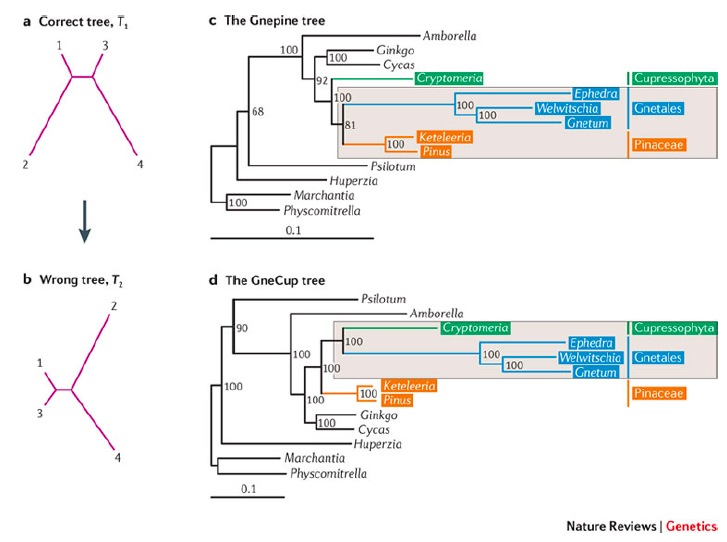
\includegraphics[width=0.5\linewidth]{figs/long-branch-attraction.png}
\caption{La atracción de ramas largas es un fenómeno que se produce cuando se infiere que los linajes que evolucionan rápidamente están estrechamente relacionados, independientemente de sus verdaderas relaciones evolutivas.}
\end{figure}
%18/09 - Patricia Álvarez
\chapter{Inferencia bayesiana (BI)}
La inferencia bayesiana se basa en la \textbf{probabilidad posterior} de un árbol condicionada por la matriz observada (alineamiento de secuencias): la probabilidad de que el árbol sea correcto dados los datos. La máxima verosimilitud examina modelos cuyos parámetros son constantes, y obtiene la verosimilitud de obtener los datos dados esos parámetros. La inferencia bayesiana también usa la verosimilitud de los datos, pero usando modelos cuyos parámetros son variables aleatorias con distribuciones estadísticas. 

Antes del análisis de los datos, se asigna una distribución inicial a los parámetros del modelo (prior), que combinada con la verosimilitud de los datos permite calcular la probabilidad posterior de dichos parámetros. El teorema de Bayes sirve para calcular esa probabilidad: la probabilidad del árbol dados los datos es la probabilidad de los datos dado el árbol (likelihood) por la probabilidad inicial del árbol (prior) entre la probabilidad de los datos a través de todos los árboles.

$$ Pr(H|D) = \frac{Pr(D|H) * Pr(H)}{Pr(D)}$$

No se puede calcular el denominador de la expresión, que es la probabilidad inicial de un árbol. Sin embargo, sí se puede aproximar la probabilidad posterior usando un procedimiento de muestreo que se acelera mediante simulaciones de Monte Carlo con cadenas de Markov (MCMC). La idea es vagar al azar en el espacio de árboles de manera que se genera una distribución de árboles cuya media es la de la distribución deseada (la probabilidad Bayesiana). Así, la inferencia bayesiana utiliza MCMC como herramienta para explorar todos los árboles posibles. Hace una buena aproximación del paisaje tras el periodo de “burnin”. Como burnin se conocen las primeras búsquedas al estar más alejadas de los árboles más probables (hay un consenso de quitar el primer 20\% de las búsquedas por este efecto). Cuanto más tiempo corre el procedimiento MCMC (más generaciones), mejor es la aproximación. Conviene repetir el proceso empezando desde diferentes puntos (random seeds).

\begin{figure}[htbp]
\centering
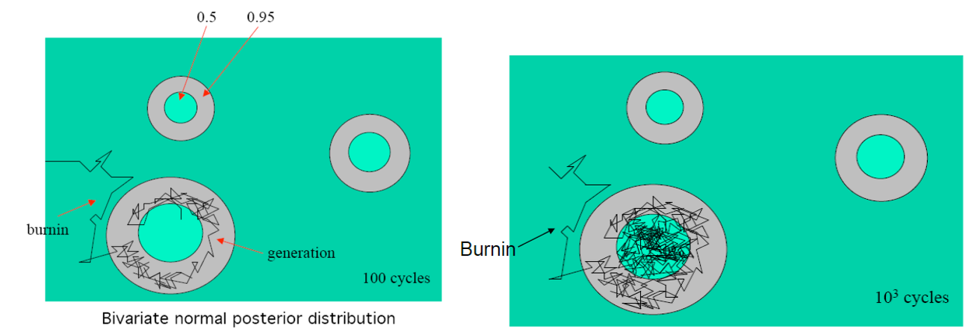
\includegraphics[width=0.5\linewidth]{figs/mcmc.png}
\caption{Aproximación del paisaje por MCMC tras 100 (izquierda) y 10000 (derecha) generaciones.}
\end{figure}

Se realizan dos búsquedas. Las cadenas frías contienen colinas altas y valles profundos. Las cadenas calientes son paisajes en los que la travesía entre colinas es más fácil. En un paisaje frío (típico de las distribuciones de parámetros) es fácil atascarse en óptimos locales. Por ello, se utilizan técnicas de mezclado para resolver el problema de los óptimos locales: se busca que las dos cadenas sean convergentes. Los criterios de convergencia son: 
\begin{itemize}
\item Las distribuciones posteriores de los parámetros del modelo son similares entre cadenas independientes.
\item Las probabilidades posteriores de los clados son similares entre cadenas independientes comenzadas con topologías aleatorias (desviación estándar promedio de las frecuencias divididas).
\end{itemize}

\begin{figure}[htbp]
\centering
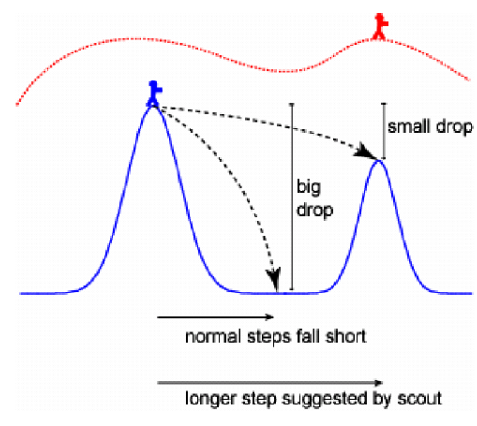
\includegraphics[width=0.5\linewidth]{figs/cadenas-frias-calientes.png}
\caption{Representación gráfica de la búsqueda de cadenas frías (azul) y calientes (rojo).}
\end{figure}

En la práctica, se empieza el procedimiento de MCMC con un árbol aleatorio y un modelo con parámetros aleatorios. En cada generación, y al azar, se propone un nuevo árbol (que se acepta o se rechaza) y un nuevo valor para los parámetros del modelo (que se acepta o se rechaza). Se ejecutan en paralelo una cadena fría y varias calentadas (que orientan a la fría a través del espacio de árboles), mediante un procedimiento MCMCMC. Cada k generaciones, se muestrea los valores de los parámetros de la cadena fría. Tras n generaciones se obtiene una distribución muestral (la cadena fría habrá pasado más tiempo en los mejores lugares del espacio de árboles) y una desviación estándar de las frecuencias divididas.

El método de inferencia Bayesiana calcula una \textbf{probabilidad posterior (BPP)} para cada nodo, que va del 0 al 1. La interpretación estadística es inmediata: es la \textbf{probabilidad de que el clado sea cierto, dado un modelo, unas premisas y unos datos}. Sin embargo, las BPP suelen ser sospechosamente altas (tendencia a la sobreestimación), mucho más que los valores de apoyo de bootstrap. Por ello, se suelen quedar con los valores bayesianos a partir de un 0.9, pero un bootstrap a partir de 70.

\begin{figure}[htbp]
\centering
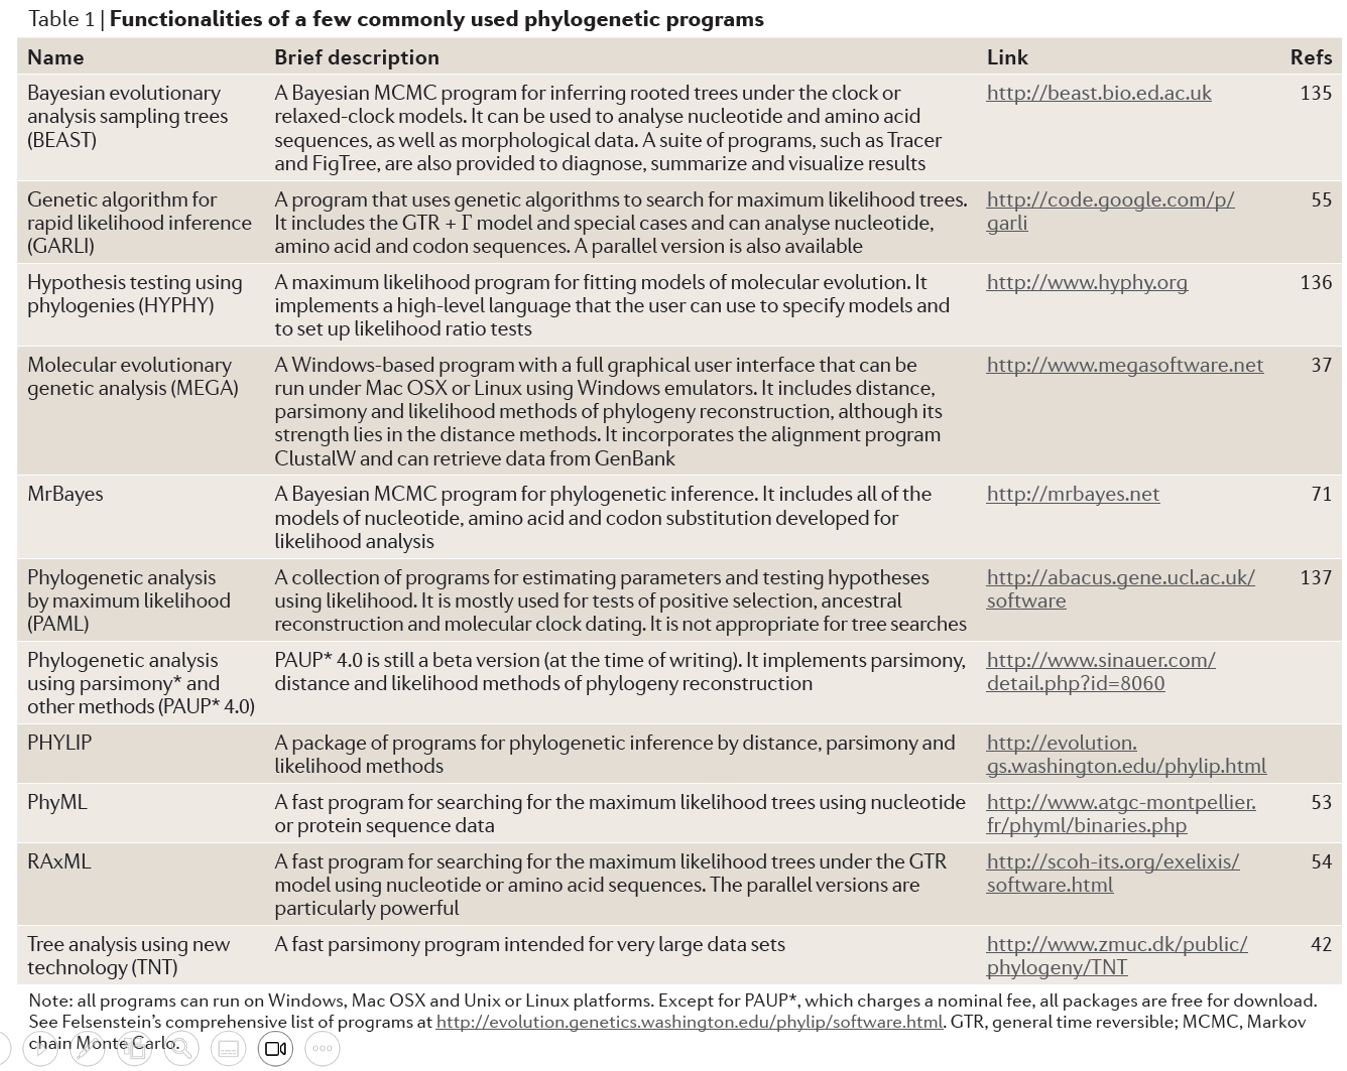
\includegraphics[width=\linewidth]{figs/programas-filogenia.png}
\caption{Lista de los programas más utilizados en filogenia.}
\end{figure}
%18/09 - Patricia Álvarez
\chapter{Cronogramas - árboles temporales}
Para estimar los años o las fechas de los cambios evolutivos de los caracteres se emplean cronogramas. La datación se basa en el reloj molecular, que a su vez se basa en la tasa de evolución de diferentes macromoléculas, ya sea ADN o proteínas. Se propone que las tasas evolutivas son constantes en el tiempo. Cada proteína o cada gen es un reloj independiente; aunque la tasa sea constante para los linajes, no es igual para todos los genes o proteínas. Para la calibración de la datación se utiliza la fecha de muestreo, la edad del fósil y los eventos biogeográficos (eventos geológicos, como apertura o cierre de océanos, movimiento de continentes, etc). Para crear estos árboles, al programa se le aportan unas estimaciones temporales, que pueden ser más estrictas (strict clock) o más relajadas (relaxed clock). Como mínimo, se debe tener una datación para el grupo externo. 

\begin{figure}[htbp]
\centering
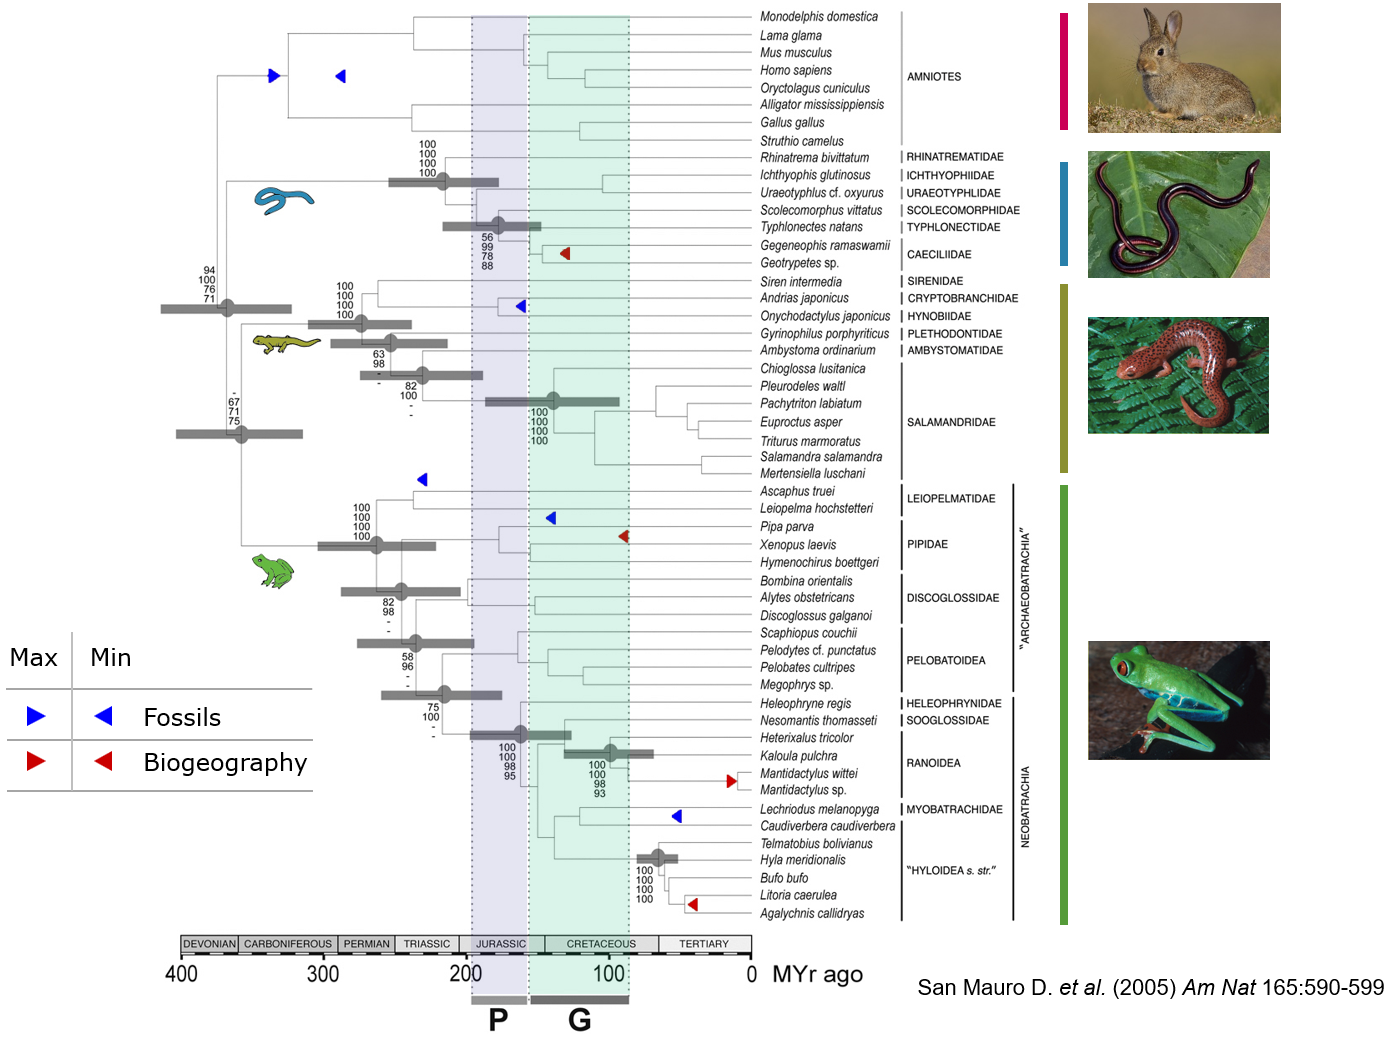
\includegraphics[width=0.9\linewidth]{figs/cronograma-ejemplo.png}
\caption{Ejemplo de cronograma. La datación se ha basado en registros fósiles (flechas azules) y eventos biogeográficos (flechas rojas).}
\end{figure}
\chapter{Resumen completo}
Un árbol filogenético tiene las especies de interés en los nodos terminales y sus relaciones mostradas por las ramas. Los nodos internos representan hipotéticos taxones extintos. Hay un grupo externo que sirve para enraizar el árbol.

\begin{figure}[htbp]
\centering
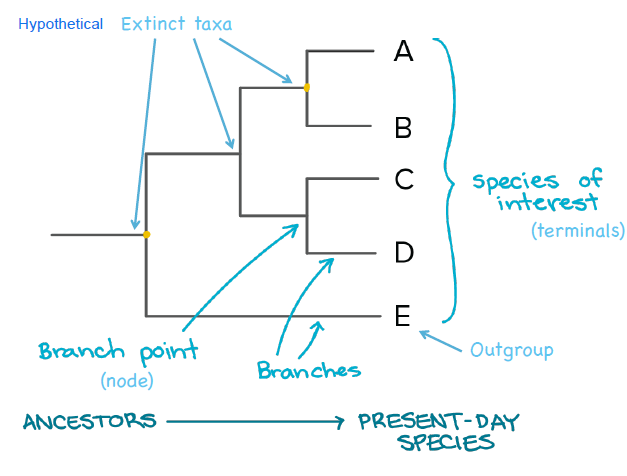
\includegraphics[width=0.7\linewidth]{figs/parts-phylotree.png}
\end{figure}

Hay distintos tipos de árbol:
\begin{itemize}
\item \textbf{Cladograma:} es una representación simple que es aceptable en matrices morfológicas. No muestra hipótesis evolutivas al no contener información sobre la relación entre ancestros y descendientes o cuánto han cambiado los descendientes a lo largo del tiempo.
\item \textbf{Filograma:} es un árbol en el que la longitud de las ramas indica la cantidad de cambios evolutivos inferidos del análisis.
\item \textbf{Cronograma:} se utiliza el tiempo para calcular las variaciones en los nodos mediante el empleo de relojes moleculares.
\end{itemize}

\begin{figure}[htbp]
\centering
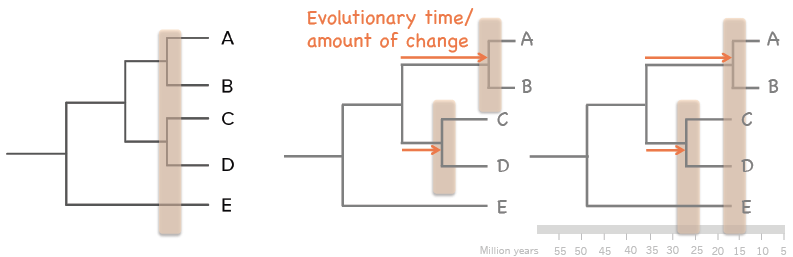
\includegraphics[width=0.7\linewidth]{figs/tree-types.png}
\end{figure}

Los árboles filogenéticos pueden tener ramas rotadas sin que cambie el mensaje. También hay distintas representaciones de los árboles que significan lo mismo. La diferencia está cuando un árbol está o no enraizado.

Se distinguen tres grupos de taxones en un árbol filogenético:
\begin{itemize}
\item \textbf{Monofilia:} todos los taxones que se originan de un mismo ancestro.
\item \textbf{Parafilia:} un ancestro, pero no todos sus descendientes.
\item \textbf{Polifilia:} algunos taxones de distintos ancestros.
\end{itemize}

\begin{figure}[htbp]
\centering
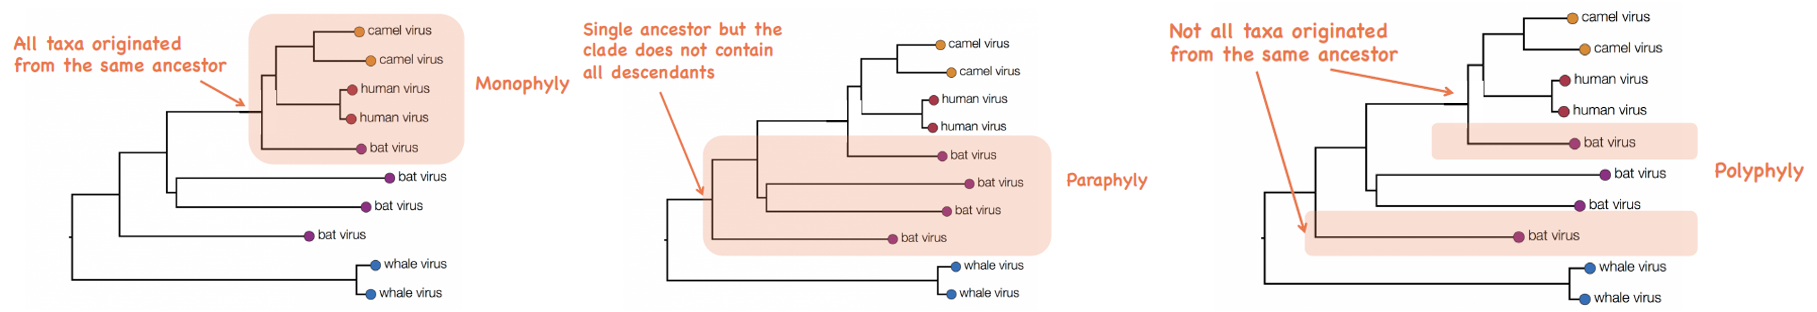
\includegraphics[width=\linewidth]{figs/tree-groups.png}
\end{figure}

Para construir un árbol filogenético, se necesitan elegir los taxones. Esto es decisión nuestra, pero hay que intentar no tener sesgos y elegir un buen ingroup y outgroup. Los tipos de datos también los podemos elegir en función de lo que está disponible. En cuanto a la cantidad de marcadores, depende del presupuesto que haya, pero se debe intentar tener los máximos posibles por PCR u otros. Se debe elegir un programa de alineamiento (MAFFT, Muscle, etc) y un modelo de evolución (jModelTest). No todos los genes evolucionan o mutan al mismo tiempo y de la misma forma, ya que depende de parámetros como el contenido GC, el tamaño genómico, el tiempo de generación, los niveles de expresión, los genes codificantes, la posición en el genoma, entre muchos otros. Por tanto, cada gen va a tener su propio modelo de sustitución, que difiere en los parámetros que describen las tasas de sustitución de cada nucleótido durante la evolución. Todas las mutaciones son posibles, pero con diferentes frecuencias dependiendo de si se trata de una transición o una transversión. Finalmente se debe elegir un método filogenético (por ejemplo, máxima verosimilitud + inferencia bayesiana) y la medición de confianza (bootstrap, convergencia, etc). 

Entre los métodos filogenéticos hay:
\begin{itemize}
\item \textbf{Máxima parsimonia:} asume que el árbol verdadero contiene el menor número de mutaciones posible, es decir, tiene la solución más parsimoniosa. Dado un set de secuencias (evidencia parcial), es necesario encontrar las secuencias ancestrales para construir un árbol enraizado y estimar el mínimo número de cambios contenidos en las ramas. No obstante, esto supone un problema computacional al no conocerse algoritmo, por lo que todos los modelos utilizan versiones simplificadas. Por ejemplo, la parsimonia ponderada emplea una puntuación diferente para cada cambio (transición/transversión) y puntuación diferente para cada posición. Para calcular la máxima parsimonia de forma manual, se emplea el algoritmo de Fitch para encontrar el estado ancestral: primero se va de descendientes al ancestro y luego del ancestro a los descendientes.
\item \textbf{Máxima verosimilitud:} la verosimilitud se define como la probabilidad de producir los datos observados por un modelo dados los parámetros. Es uno de los métodos más poderosos al poder utilizar modelos de sustitución (modelos evolutivos), corrige múltiples sustituciones y permite estimar la longitud de la rama, que indica la cantidad de cambios desde el ancestro. El problema de la máxima verosimilitud es la atracción de las ramas largas, un fenómeno que se produce cuando se infiere que los linajes que evolucionan rápidamente están estrechamente relacionados, independientemente de sus verdaderas relaciones evolutivas.
\item \textbf{Inferencia bayesiana:} basado en el teorema de Bayes, el enfoque bayesiano combina la probabilidad a priori de un árbol P(A) con la probabilidad de los datos (B) para producir una distribución de probabilidad posterior de los árboles P(A|B). La verosimilitud da la probabilidad de los datos dada la hipótesis y la bayesiana le da la probabilidad de la hipótesis dados los datos. Por ello, se habla de probabilidad posterior, y utiliza el algoritmo MCMC. Este algoritmo empieza en algún sitio, el cual tiene una verosimilitud y una probabilidad previa. Aleatoriamente se propone un nuevo estado (ajustando la longitud de una rama), y si la verosimilitud * probabilidad previa mejora, la cadena va allí. Después se calcula la relación de la probabilidad posterior entre el estado actual y el estado previo, que es entre 0 y 1. Se elije un número aleatorio entre esos valores y, si ese número tiene una probabilidad mejor que la relación de estados, se acepta el cambio. Así es como la cadena atraviesa los valles de probabilidad.
\end{itemize}

\begin{figure}[htbp]
\centering
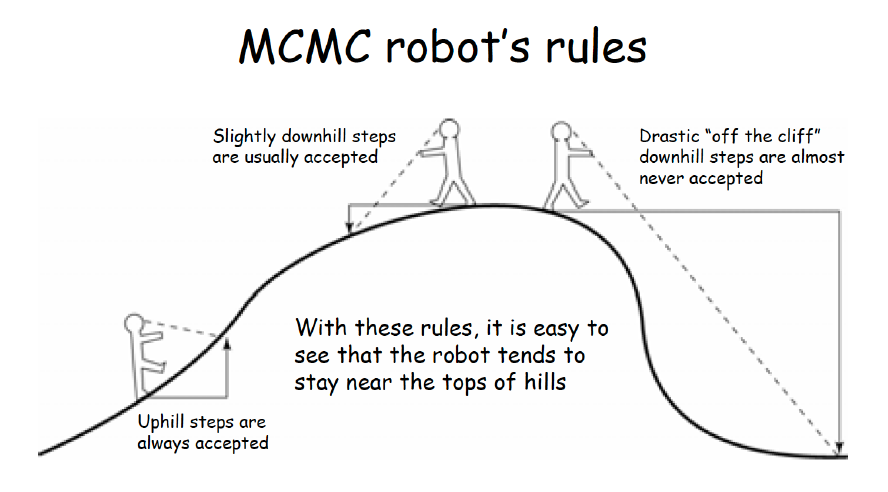
\includegraphics[width=0.6\linewidth]{figs/mcmc-rules.png}
\end{figure}

También hay varias maneras de evaluar la confianza:
\begin{itemize}
\item \textbf{Soporte de Bremer [> 70\%]:} diferencia en las longitudes de las ramas cuando se eliminan los clados (solo en parsimonia).
\item \textbf{Jackknife [> 70\%]:} probabilidad de que un clado se observe en todos los árboles (parsimonia).
\item \textbf{Bootstrap [> 70\%]:} probabilidad de que un clado se observe en todos los árboles (máxima verosimilitud).
\item \textbf{Probabilidad posterior [> 0.95]:} probabilidad de que un clado sea asignado bajo las condiciones muestradas (inferencia bayesiana).
\item \textbf{Convergencia:} evaluar si todas las cadenas (MCMC) convergen en la misma
solución (inferencia bayesiana).
\end{itemize}
%18/09 - Patricia Álvarez
\chapter{Ejercicios tipo examen}
\section{Ejercicio 1: Construir un árbol a partir de un alineamiento.}
Dado el siguiente alineamiento, construye un árbol filogenético. 
\begin{table}[h]
\centering
\begin{tabular}{l | l l l l }
\hline
& 1 & 2 & 3 & 4 \\
\hline
A & a & a & a & b\\
B & a & a & a & b \\
C & b & a & a & b \\
D & b & b & a & a \\
E & b & b & a & a \\
F & b & b & b & b
\end{tabular}
\end{table}

Hay varias formas de empezar. Una de ellas sería por aquellos que son iguales. Los taxones A y B son iguales, al igual que D y E. Por tanto, sabemos que esos taxones van juntos. Después, se busca el taxón más similar. En este caso, el taxón C es el siguiente más similar a los taxones A y B. Por último, el taxón F es el más diferente, siendo por tanto el outgroup. En resumen, el árbol quedaría así:

\begin{figure}[htbp]
\centering
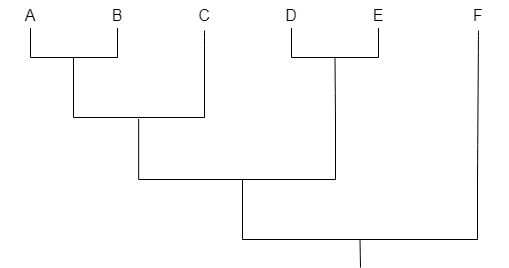
\includegraphics[width=0.7\linewidth]{figs/phylotree1.drawio.png}
\end{figure}

\section{Ejercicio 2: Construir la matriz de caracteres desde un árbol.}
Dado el siguiente árbol filogenético con las distintas mutaciones, construye una matriz de alineamiento.
\begin{figure}[htbp]
\centering
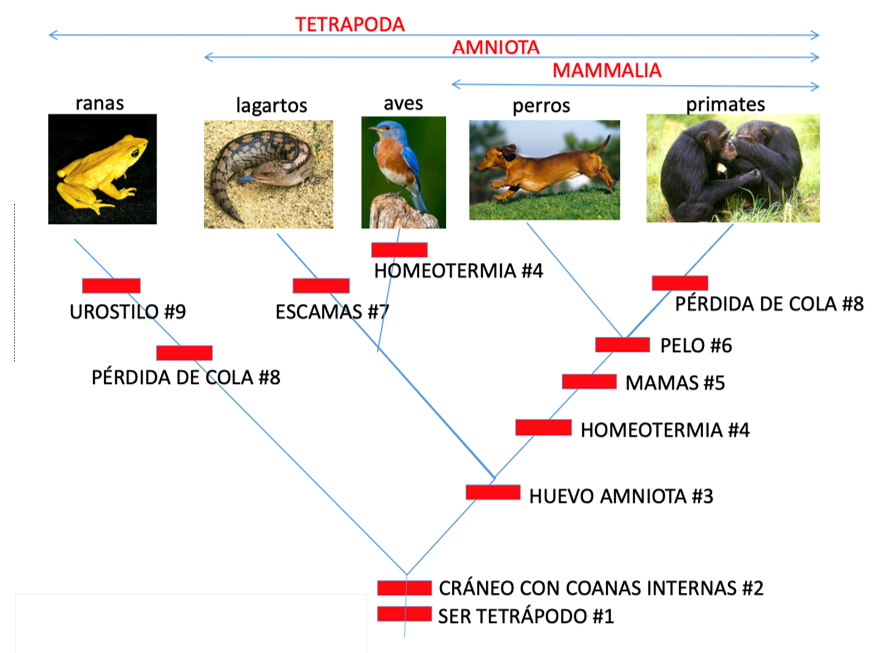
\includegraphics[width=0.7\linewidth]{figs/ejercicio-2.png}
\end{figure}

\begin{table}[htbp]
\centering
\begin{tabular}{l | l l l l l l l l l }
\hline
& 1 & 2 & 3 & 4 & 5 & 6 & 7 & 8 & 9 \\
\hline
Ranas & a & a & b & b & b & b & b & a & a\\
Lagartos & a & a & a & b & b & b & a & b & b\\
Aves & a & a & a & a & b & b & b & b & b\\
Perros & a & a & a & a & a & a & b & b & b\\
Primates & a & a & a & a & a & a & b & a & b
\end{tabular}
\caption{Matriz de alineamiento. La a indica presencia, la b indica ausencia}
\end{table}

\section{Identificación de caracteres}
En relación con el árbol filogenético del ejercicio 2, explica los caracteres en relación con todos los integrantes del árbol.

Los caracteres 1 y 2 son plesiomorfías al ser ancestrales. El carácter 3 es una sinapomorfía (sería una simplesiomorfía para los amniotas, pero como nos piden relacionarlo con todos los taxones, es una sinapomorfía del árbol). El carácter 9 es una autapomorfía de las ranas, y el 7 de los lagartos. El carácter 8 es otra autapomorfía con convergencia entre ranas y primates, generando así un grupo polifilético (el ancestro común más cercano no tiene el carácter). 

El grupo hermano de los amniotas son las ranas. Así, el grupo hermano de los mamíferos son lagartos y aves; no son los amniotas porque los mamíferos están englobados en los amniotas.  

\end{document}
